
\subsection{Studies in the General Phase Space} % (fold)
\label{sub:coarse_studies}

In order to evaluate the overall discrimination performance of the DNNs to that of the physics-driven variables, we examine the ROC curves in Figure~\ref{fig:combinedROC1}. In particular, we compare the DNNs to $n$-subjettiness~\cite{nsub} $\tau_{21} = \tau_{2}/\tau_{1}$, the jet mass, and the distance $\Delta R$ between the two leading $p_{T}$ subjets.  In Figure~\ref{fig:combinedROC1a}, we can see that the three DNNs have similar performance, but the MaxOut networks outperforms the ConvNet networks.  We suspect that the MaxOut outperforms the ConvNets due to sparsity of the jet-images, whereby the MaxOut network views the full jet-image from the inital hidden layer while the sparsity tends to make it difficult for the ConvNets to learn meaningful convolution filters.  We also see that the ConvNet-Norm outperforms the ConvNet trained on the un-normalized jet-images.  We observe that the classification performance of the ConvNet discriminant is highest when jet images are normalized, despite the fact that image normalization destroys jet mass information from the images. As we will see soon, it is difficult for these networks to fully learn the jet mass, so the lack of of mass information from pre-processing does not necessarily lead to worse discrimination performance. On the other hand, normalization is having an impact on the ability to effectively train the ConvNet network on jet images.  Finally, we see that the DNNs significantly improve the discrimination power relative to the Fisher-Jet discriminant\footnote{The Fisher discriminant is trained in three partitions of $\Delta  R$ ($\Delta R \in [0.25, 0.5],\ [0.5, 0.75],\ [>0.75])$, in order to account for the non-linear variation in jet-images from the differing positions of the two subjets.  Also note that unlike in the original implementation, here we do not normalize the jet images when computing the Fisher Jet.  This leads to slightly better performance.}, as described in reference~\cite{Cogan:2014oua}. In addition, in Figure~\ref{fig:combinedROC1b} we see that the DNNs also outperform the two-variable combinations of the physics inspired variables (computed using the 2D likelihood ratio\footnote{This is computed using the same regulated binning scheme as the 1D likelihoods described earlier.}).   It is interesting to note that combining mass and $\tau_{21}$, or $\tau_{21}$ and $\Delta R$, achieve much higher performance than the individual variables and are significantly closer to the performance of the DNNs.  However, the large difference in performance between the DNNs and the physics-variable combinations implies the DNNs are learning information beyond these physics variables.
%This is likely due to the normalization and energy binning helping to provide more uniformity in the typical pixel intensities across jet-images.
\begin{figure}[!htbp]
\begin{center}
\subfloat[]{
	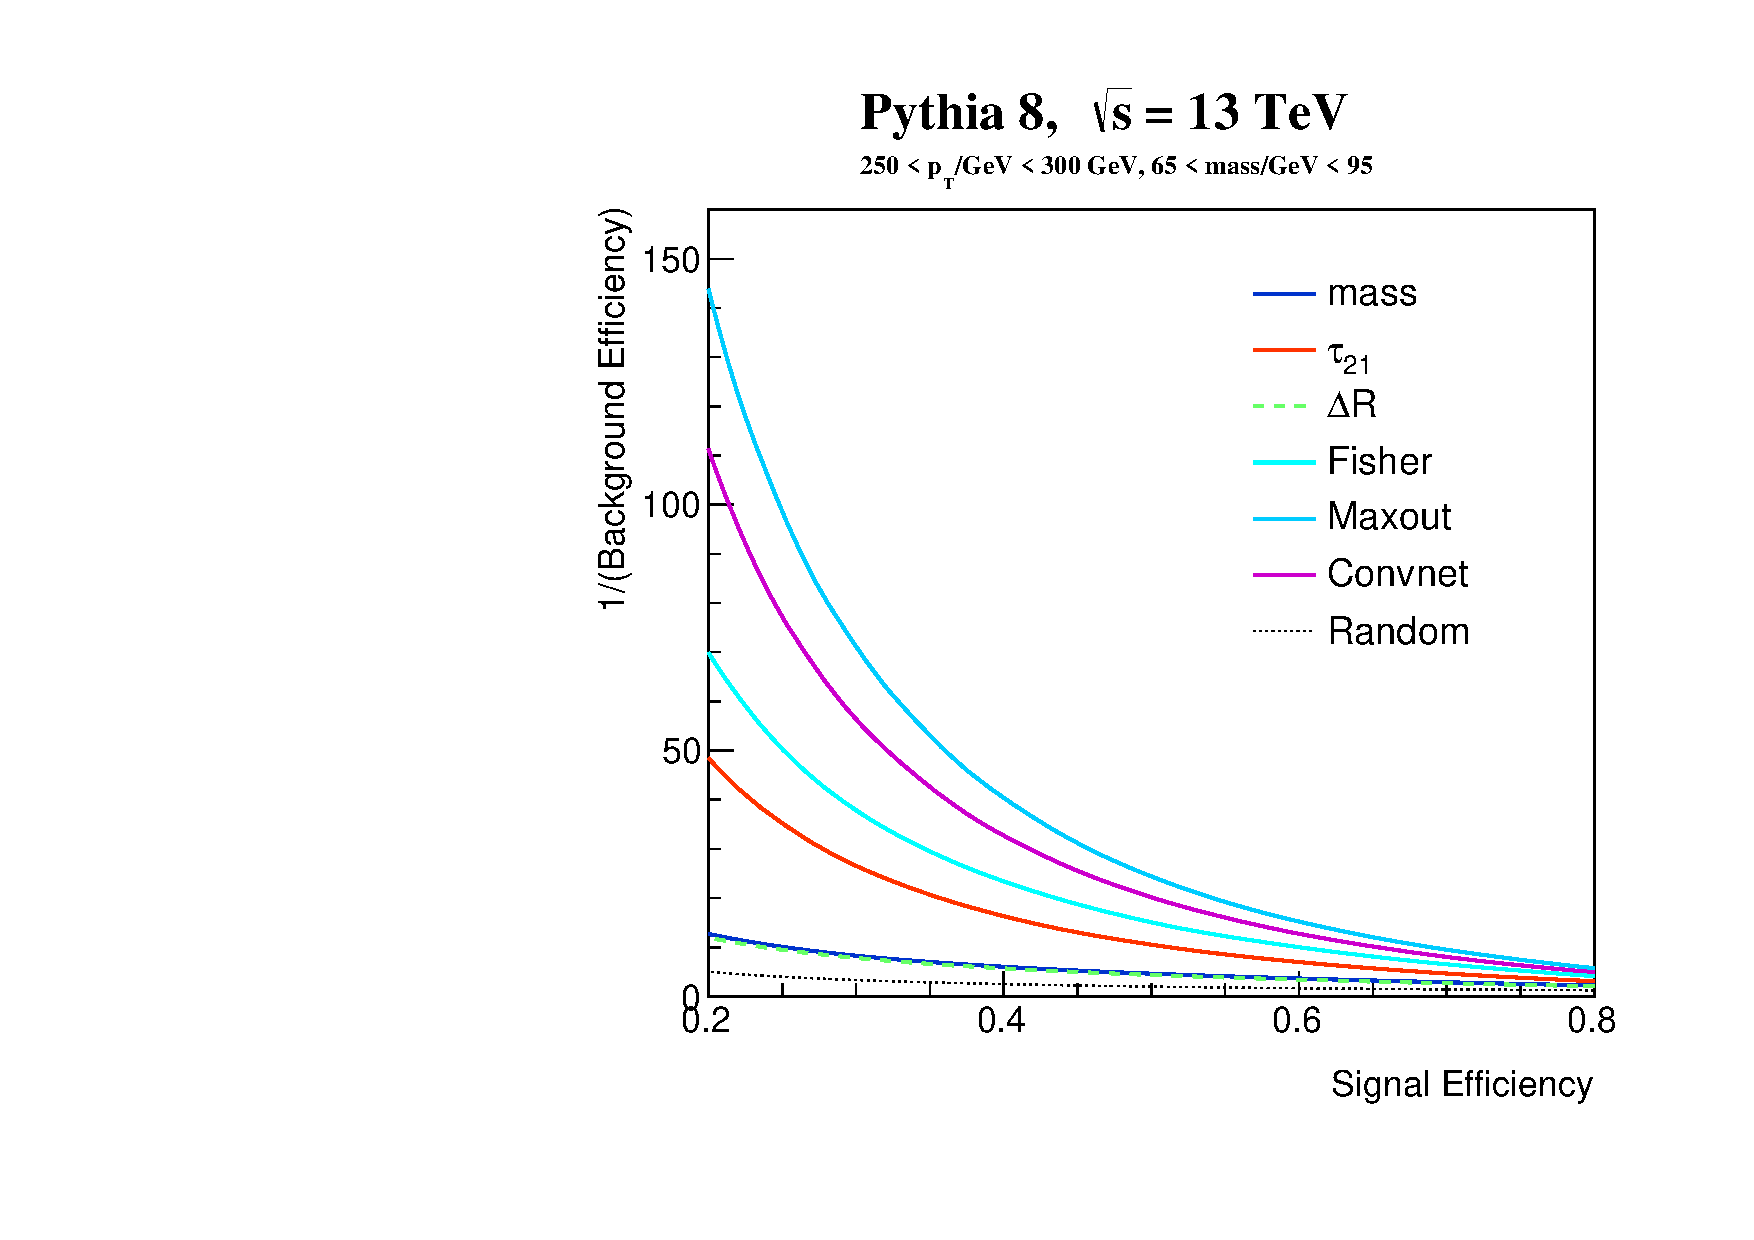
\includegraphics[width=0.48\textwidth,angle=0]{figures/ROC_1}
	\label{fig:combinedROC1a}
}
\subfloat[]{
	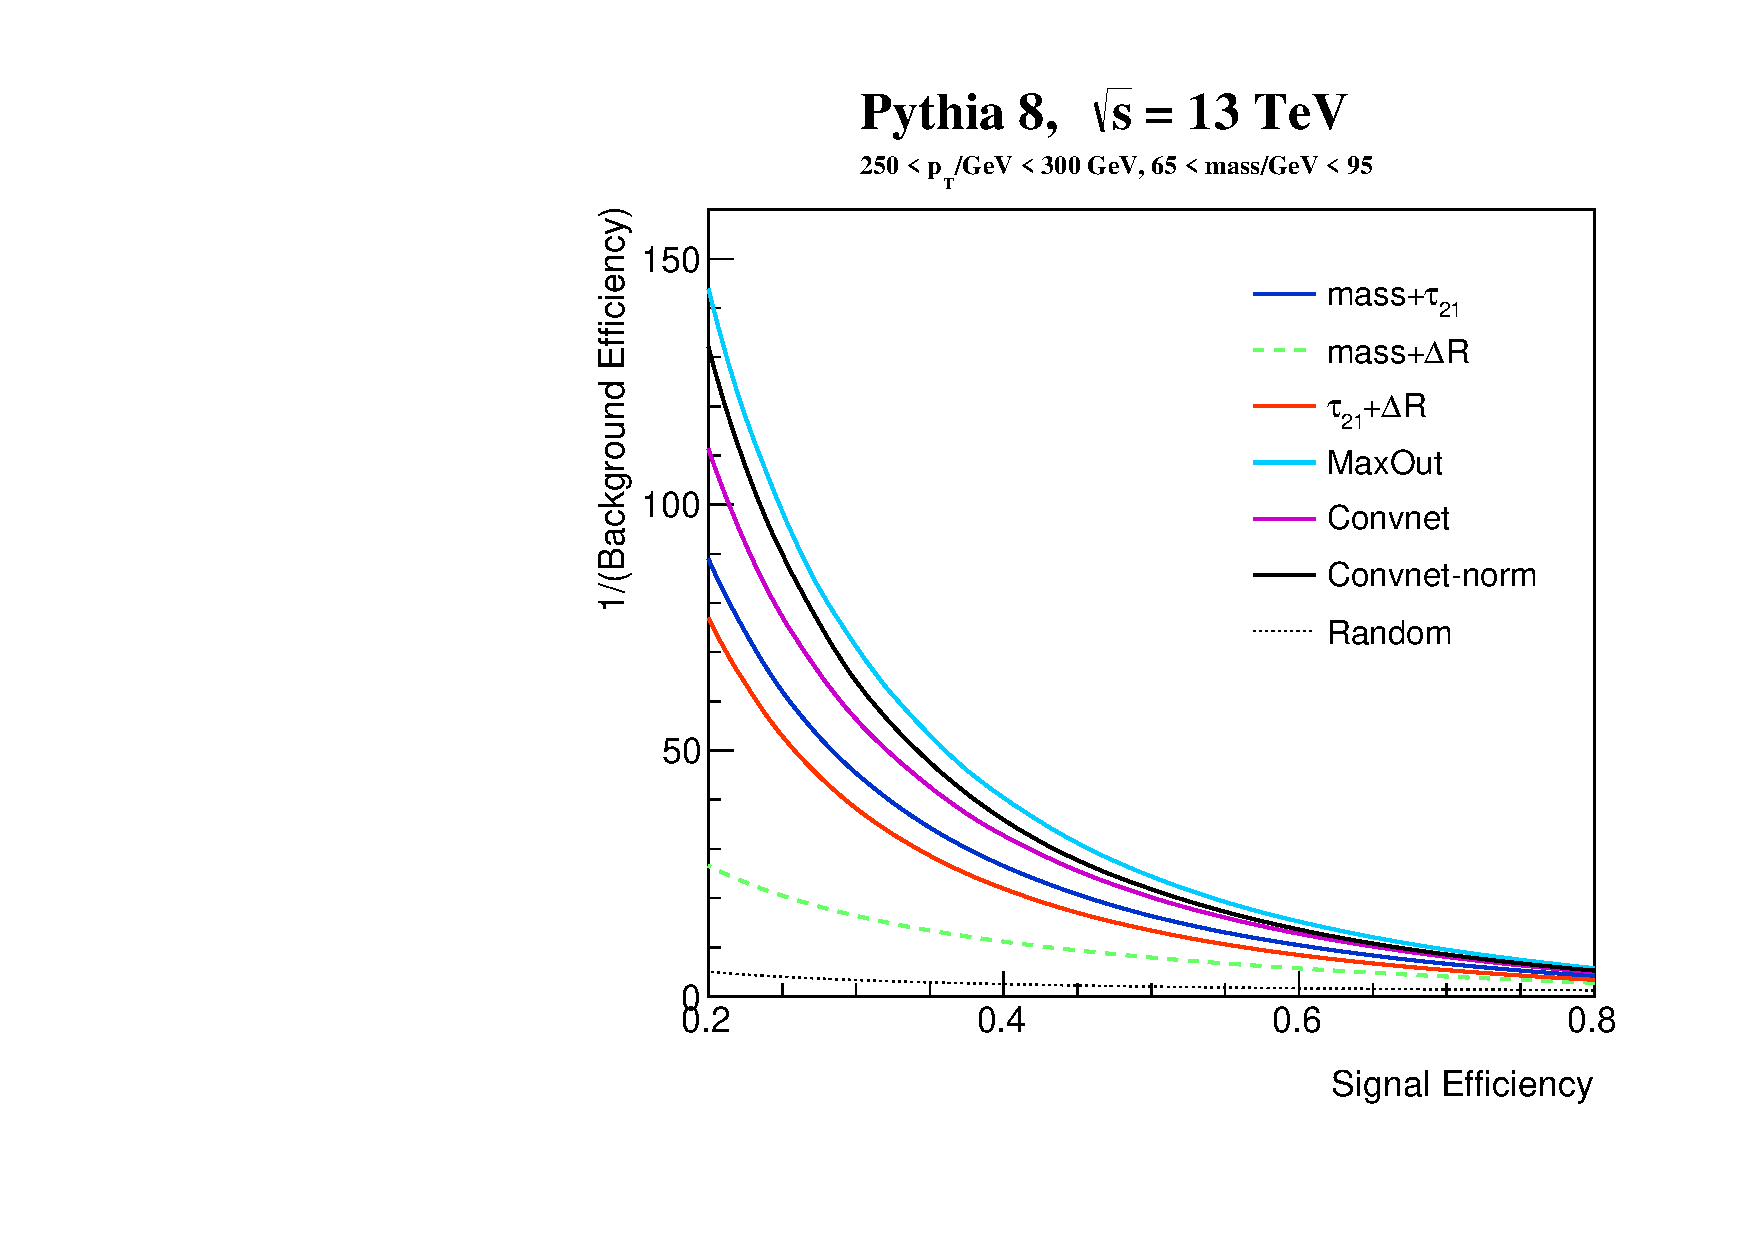
\includegraphics[width=0.48\textwidth,angle=0]{figures/ROC_2}
	\label{fig:combinedROC1b}
}
\end{center}
   \caption{Left: ROC curves for individual physics-motivated features as well as three deep neural network discriminants.  Right: the DNNs are compared with pairwise combinations of the physics-motivated features.}
  \label{fig:combinedROC1}
\end{figure}


While we can see in Figure~\ref{fig:combinedROC1} that the DNNs outperform the individual and two-variable physics inspired discriminators, we want to understand if these physics variables have been learned by the networks.  As such, we compute the combination of the DNNs with each of the physics inspired variables (using the 2D likelihood), as seen for the ConvNet in Figure~\ref{fig:combinedROC2a} and for the MaxOut network in Figure~\ref{fig:combinedROC2b}. In both cases, we see that the discriminators combining $\Delta R$ or $\tau_{21}$ with the DNNs does not improve performance.  This indicate that the discriminating information in these variables relevant for the classification task has already been fully learned by the networks\footnote{This is not strictly speaking true, since there may be other variables that are needed in order to fully capture the full information of a given variable.  For example, consider independent random variables $X_i$ that are $\pm 1$ with probability $1/2$.  If $Y=X_1X_2$, then $X_1$ is independent of $Y$ but the joint distribution of $(X_1,X_2)$ is not independent of $Y$.  The statement is true in the absence of interactions with other variables.}.  However, adding mass in combination with the DNNs shows a noticeable improvement in performance over the DNNs alone.  This indicates that not all of the discriminating information relevant for jet tagging contained in the mass variable has been learned by the DNNs.  While it is not shown, similar patterns are found for the Convnet-Norm network.
\begin{figure}[!htbp]
  \begin{center}
\subfloat[]{
	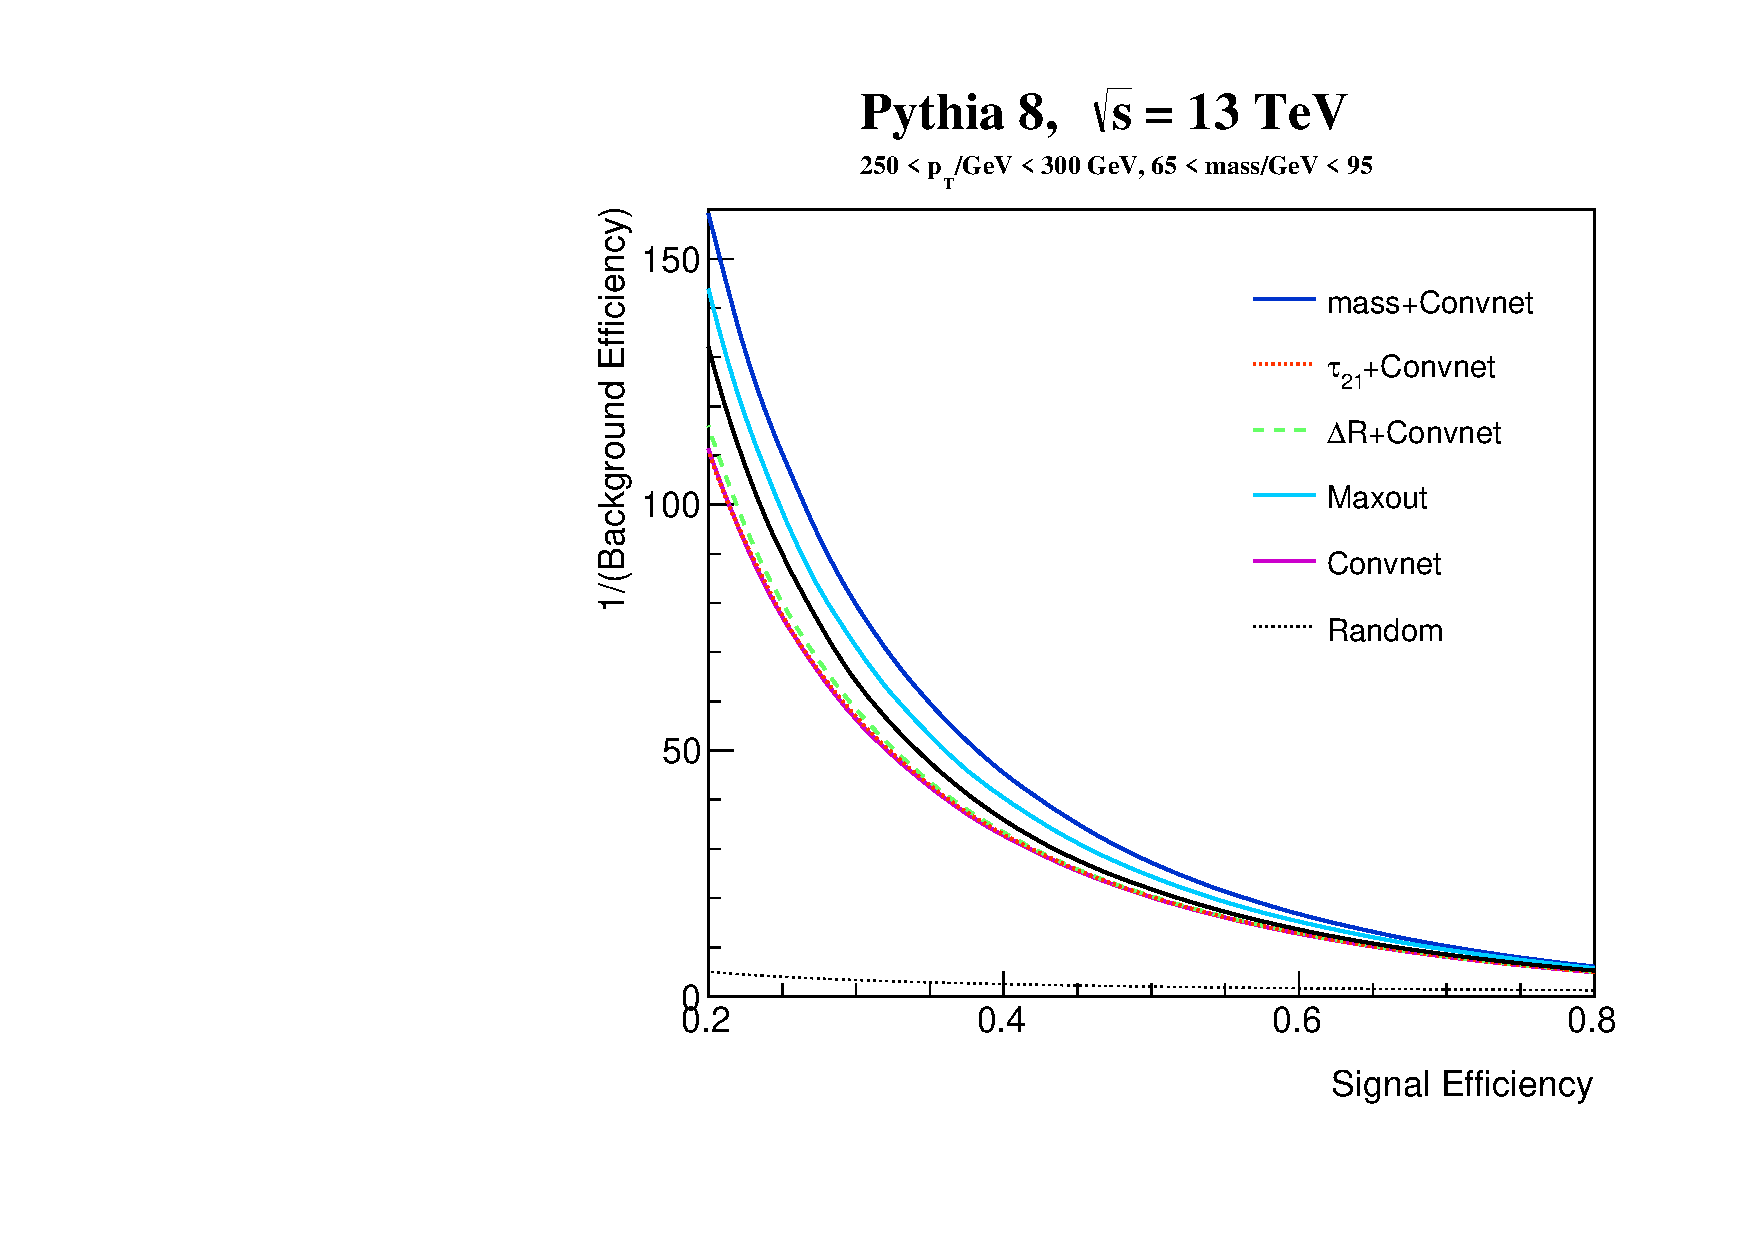
\includegraphics[width=0.48\textwidth,angle=0]{figures/ROC_3}
	\label{fig:combinedROC2a}
}
\subfloat[]{
	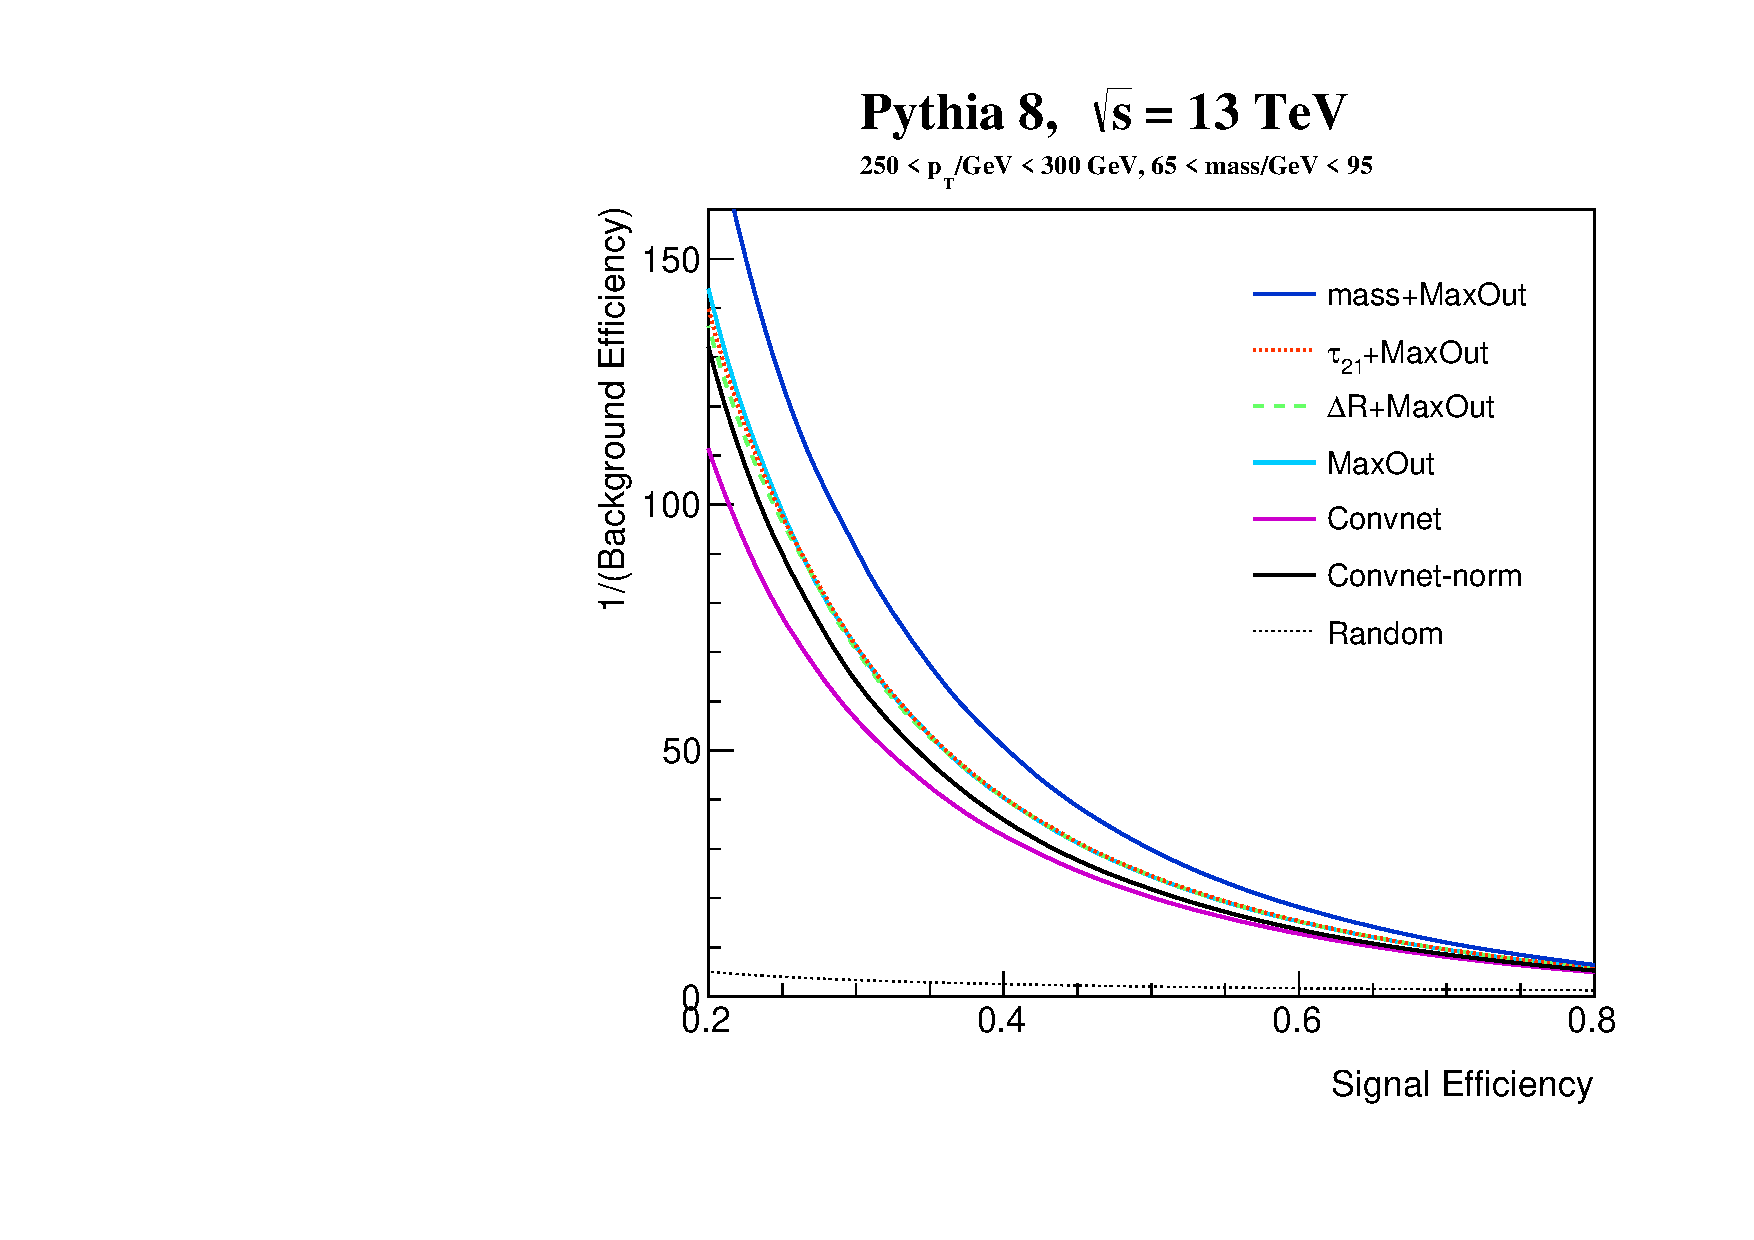
\includegraphics[width=0.48\textwidth,angle=0]{figures/ROC_4}
	\label{fig:combinedROC2b}
}
\end{center}
  \caption{ROC curves that combined the DNN outputs with physics motivated features for the Convnet (left) and MaxOut (right) architectures.}
  \label{fig:combinedROC2}
\end{figure}

The conditional distributions between the DNN output and the physics-variables are shown in Figure~\ref{fig:sculptedConv} for the ConvNet, and in Figure~\ref{fig:sculptedMax} for the MaxOut network, against the jet mass, $\Delta R$, and $\tau_{21}$.   These distributions are normalized in bins of the DNN output, and thus the $z$-axis shows a discretized estimate of the conditional probability density of a physics variable value given the network output (i.e. $\Pr(\text{variable}|\text{network output})$). Normalizing the distributions in this way allows us to see the most probable values of the physics variables at each point of the network output, without being affected by the overall distribution of jets in this 2D space.  We can see that both networks show a strong non-linear relationship with $\tau_{21}$ and $\Delta R$, giving further evidence that this information has been learned by the networks.  However, the correlations are much weaker with the jet mass variable, being slightly more strongly correlated with the MaxOut network output.  While it is not shown, similar patterns are found for the Conv-Norm network.   For reference, the full joint distributions can be found in Appendix~\ref{sec:app:dists}. 
\begin{figure}[htbp!]
  \begin{center}
  
  \subfloat[ ConvNet\label{fig:sculptedConv}]
      {
        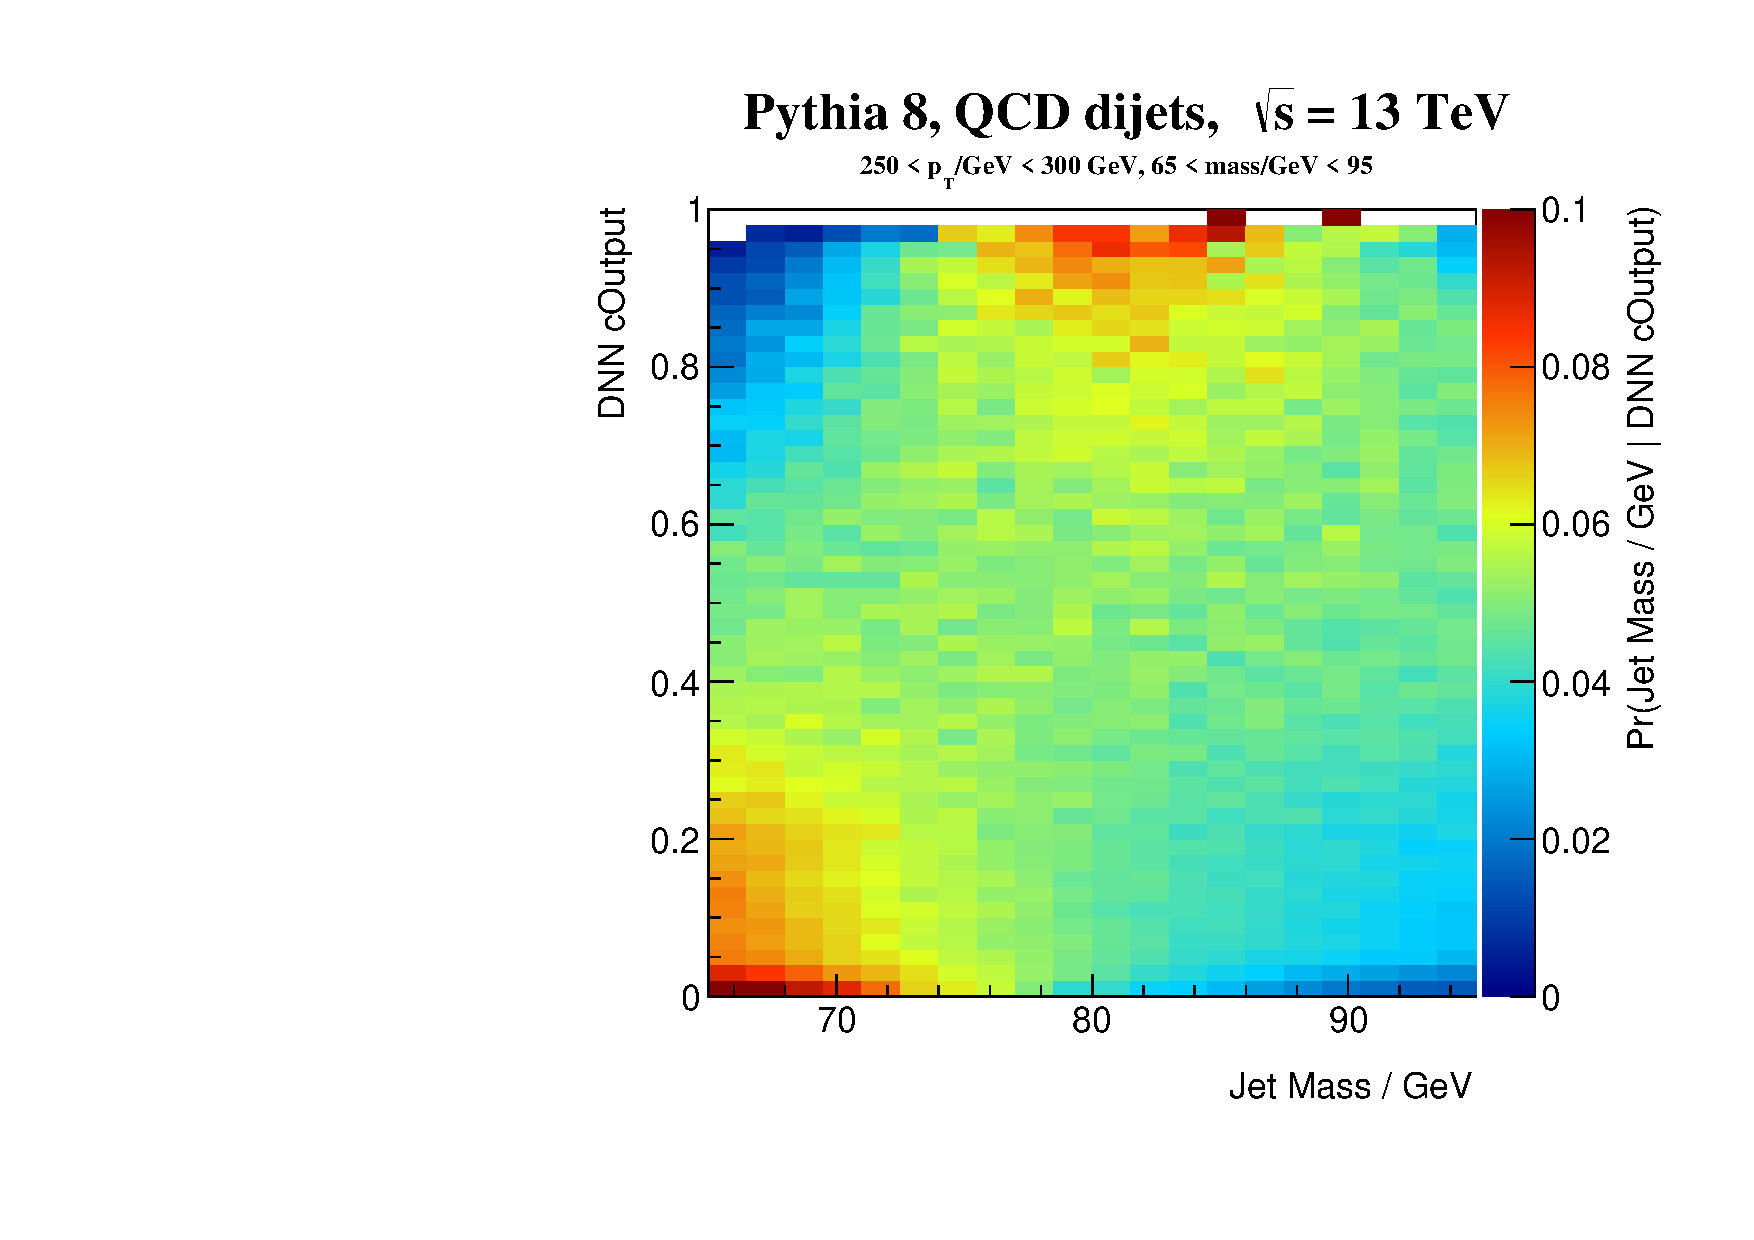
\includegraphics[width=0.32\textwidth]{figures/mass_convnet_back_norm_invert.pdf}
         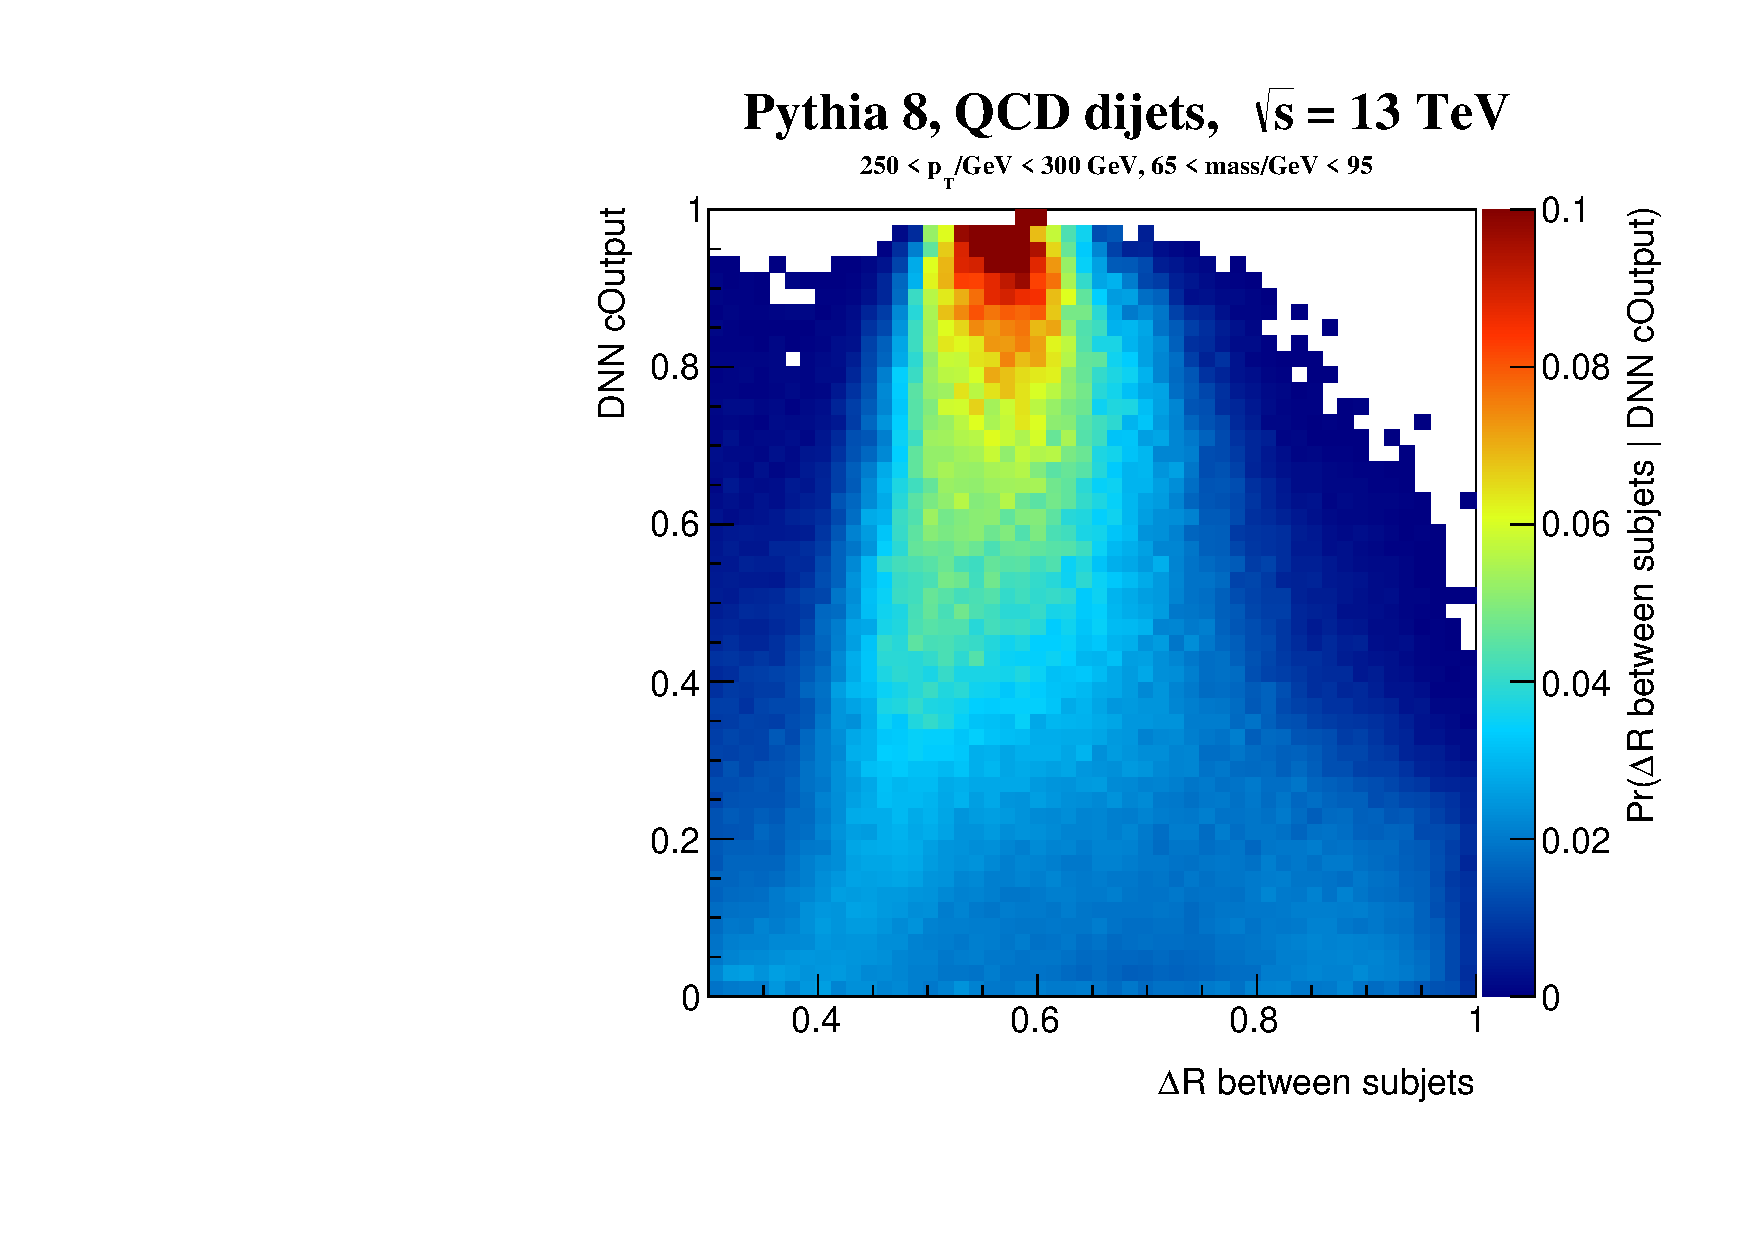
\includegraphics[width=0.32\textwidth]{figures/dR_convnet_back_norm_invert.pdf} 
         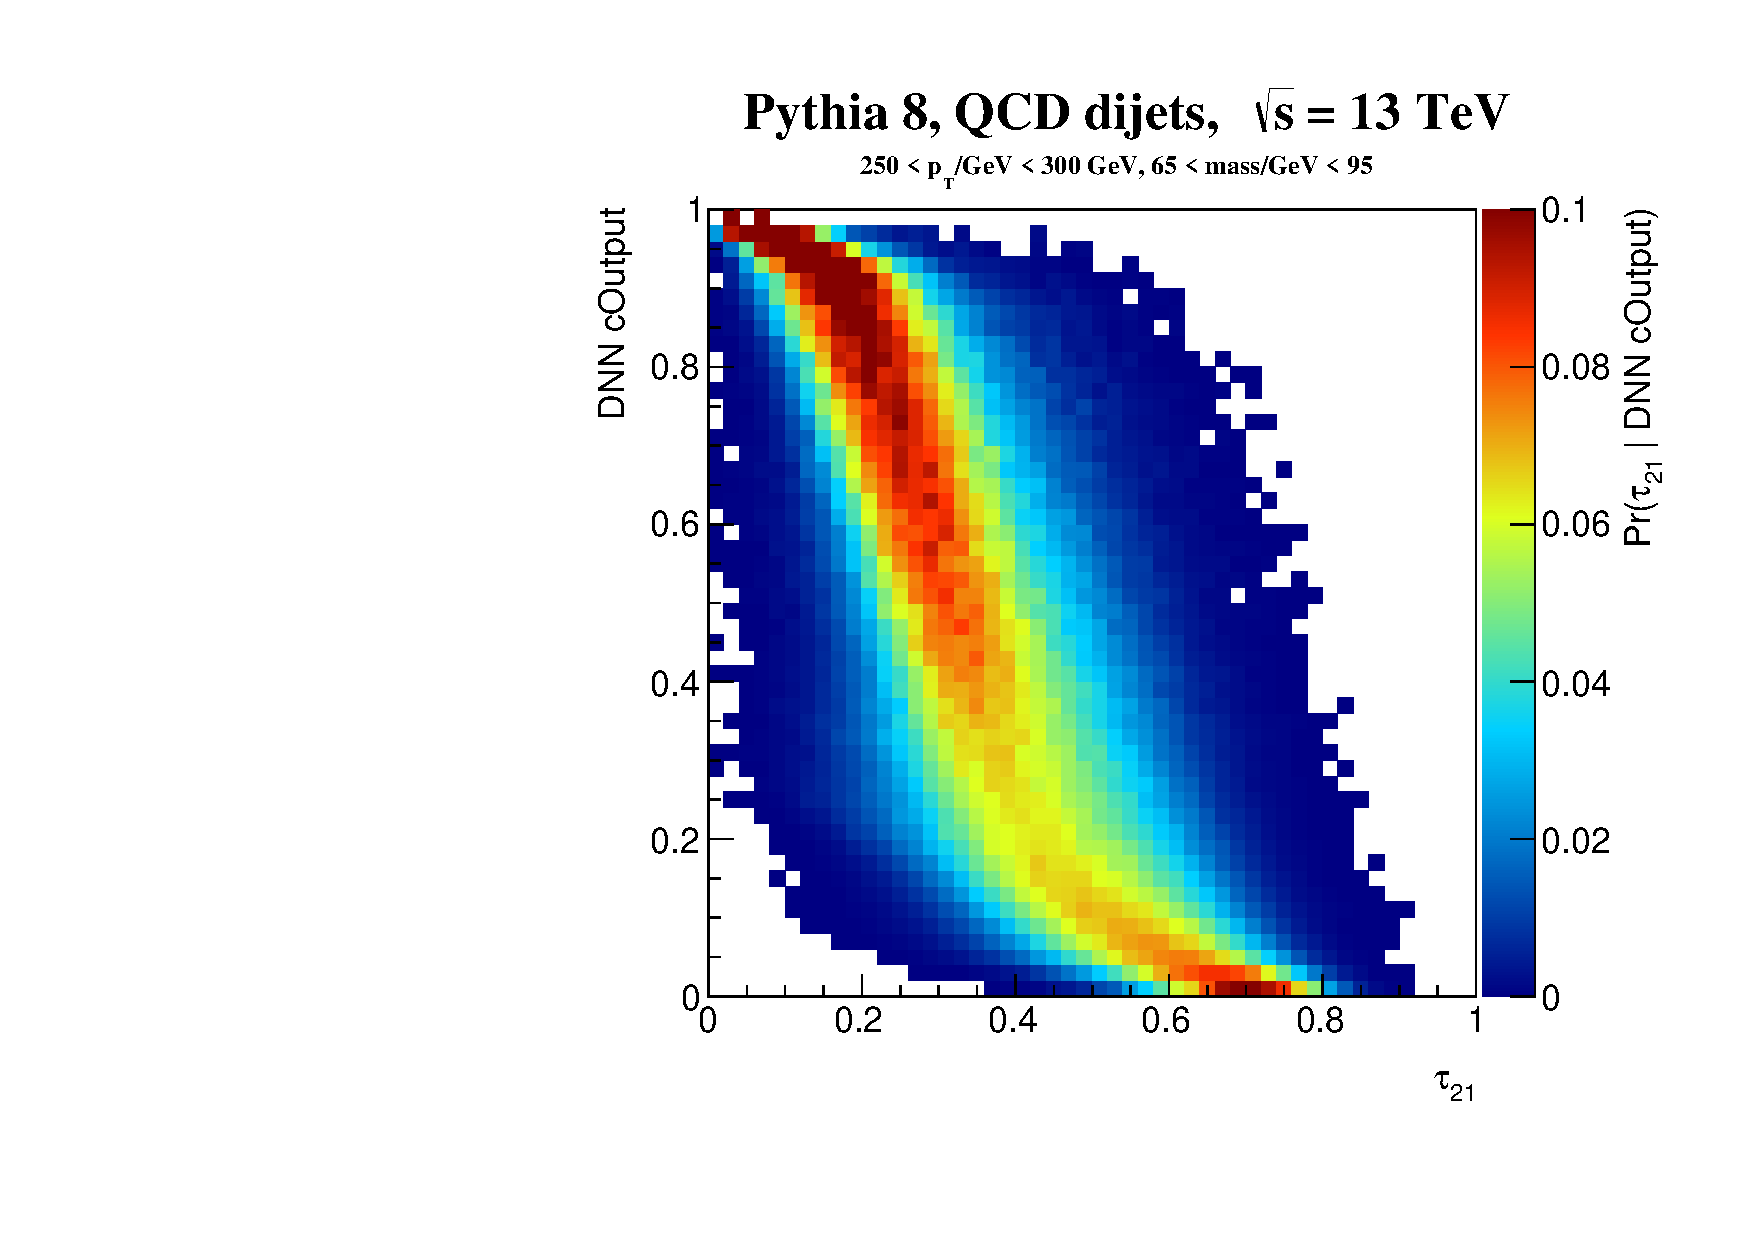
\includegraphics[width=0.32\textwidth]{figures/tau21_convnet_back_norm_invert.pdf}
      }\\
        \subfloat[MaxOut\label{fig:sculptedMax}]
      {
        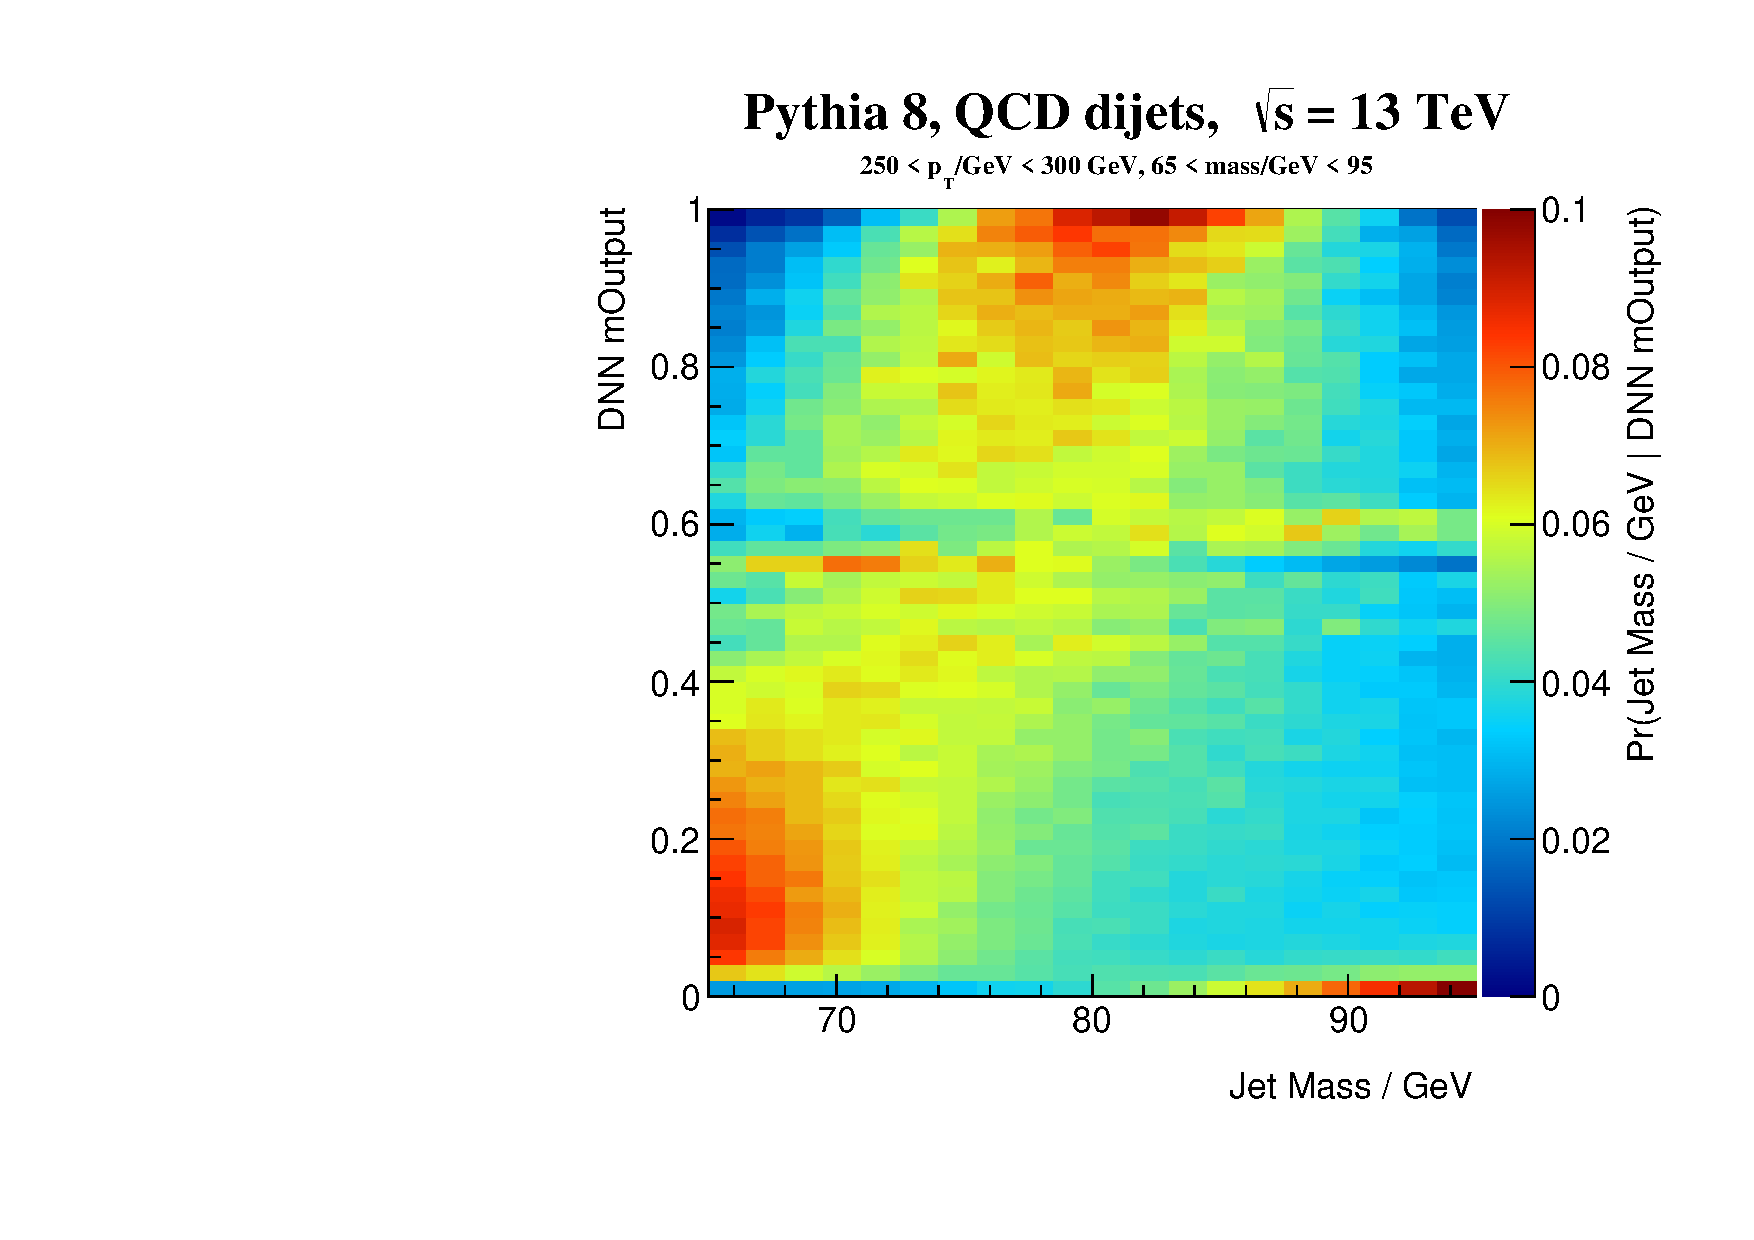
\includegraphics[width=0.32\textwidth]{figures/mass_maxout_back_norm_invert.pdf}
         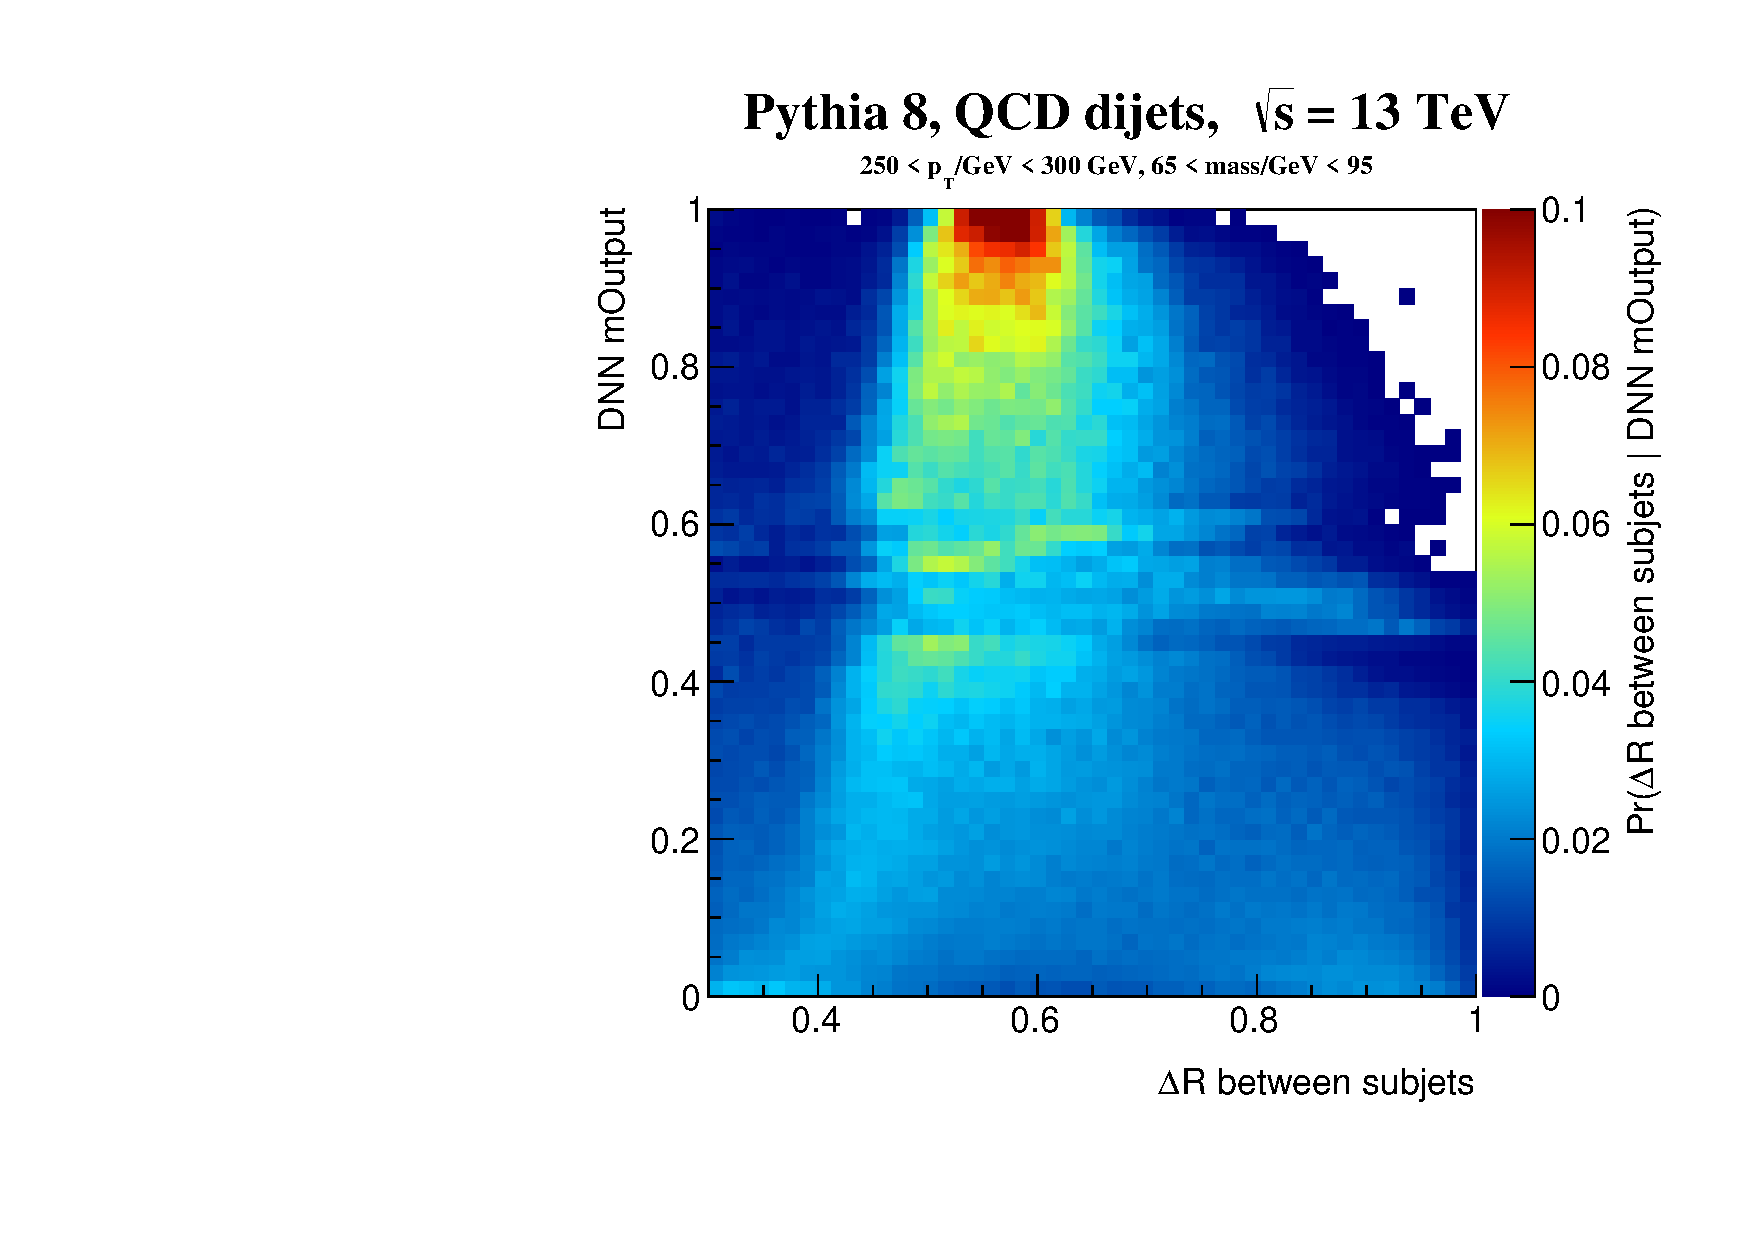
\includegraphics[width=0.32\textwidth]{figures/dR_maxout_back_norm_invert.pdf} 
         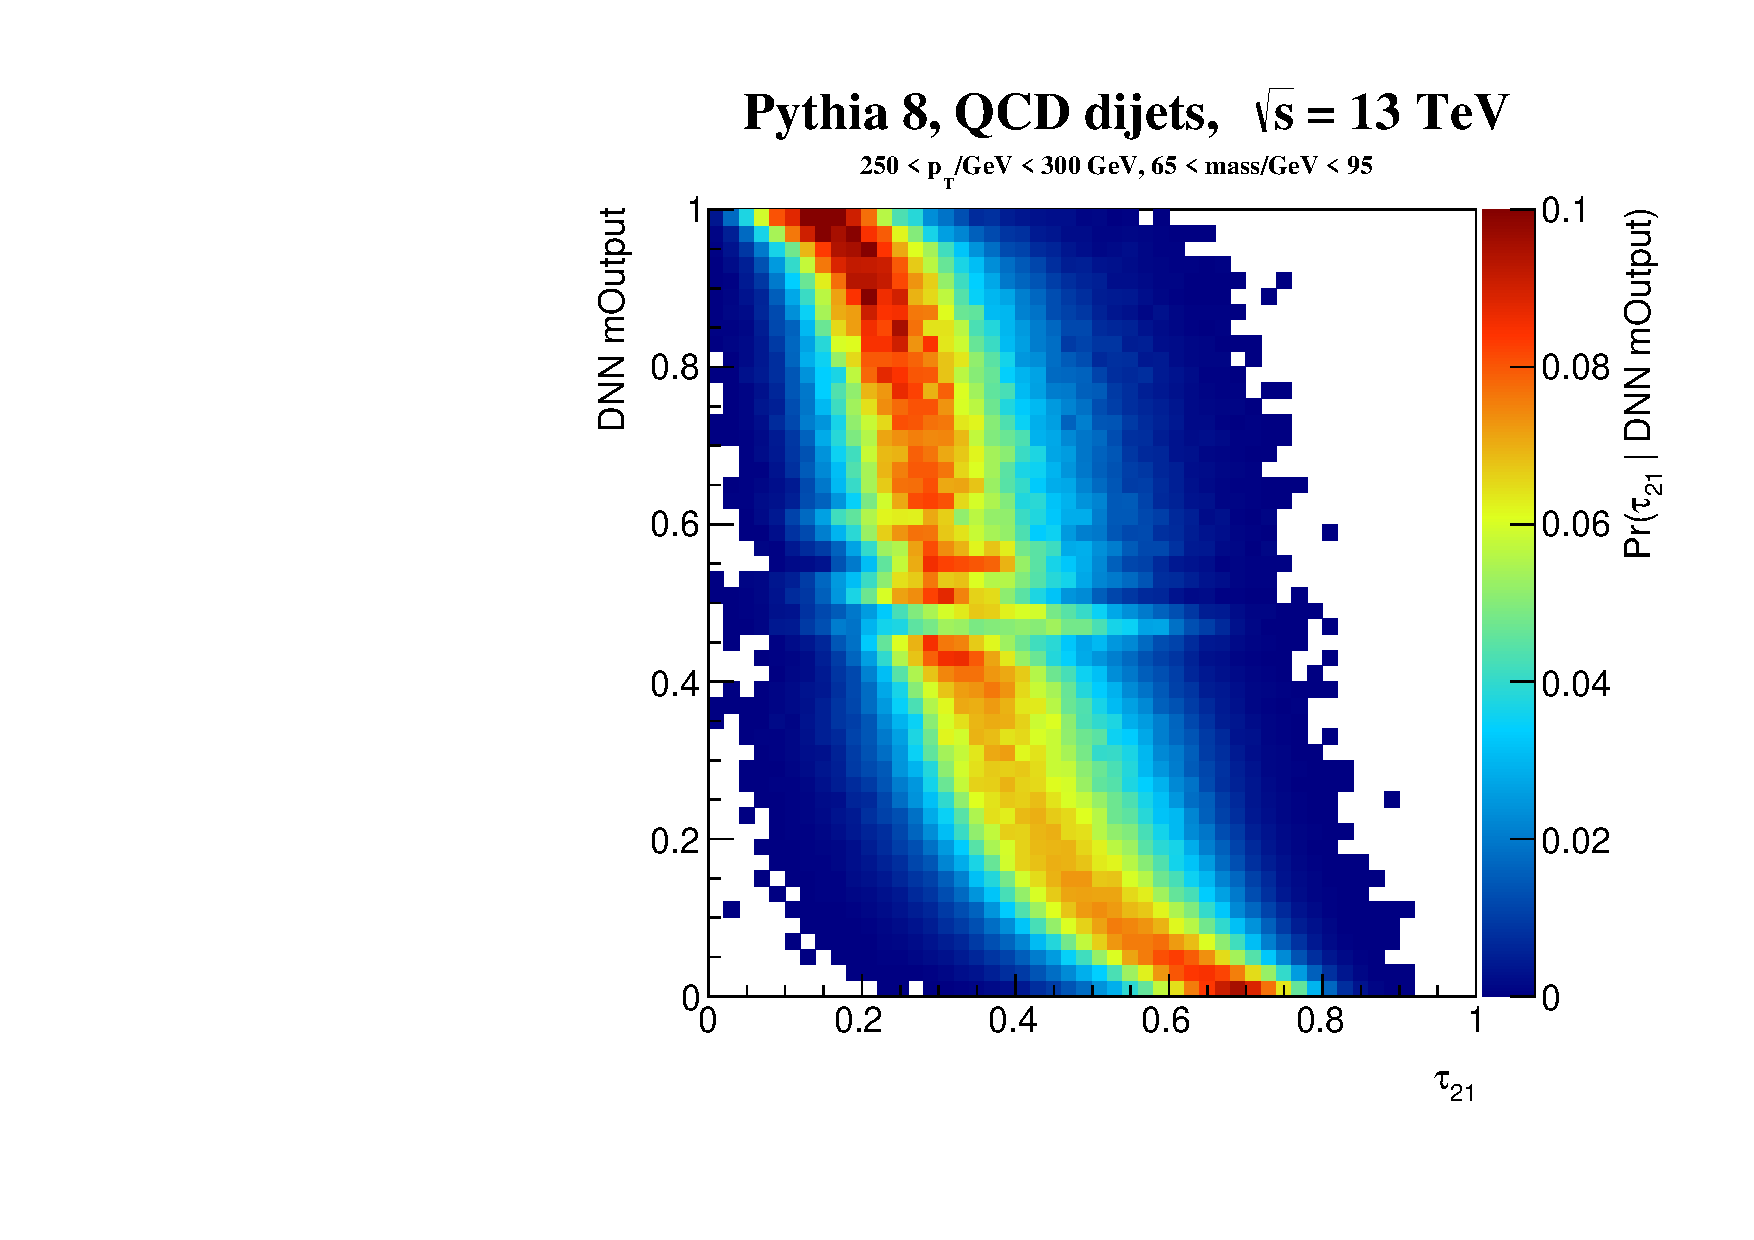
\includegraphics[width=0.32\textwidth]{figures/tau21_maxout_back_norm_invert.pdf}
      }\\

      \caption{Network output versus mass (left), $\Delta R$ (middle), and $\tau_{21}$ (right) for the ConvNet (top) and MaxOut (bottom) networks.  Each row is normalized and represents the probability distribution of the variable shown on the x-axis given the network output.}
      \label{fig:qcdsculpt}

    \end{center}
\end{figure}

\subsection{Understanding what is learned} % (fold)
\label{ssub:understanding_what_is_learned}

In order to gain a deeper understanding of the physics leaned by the DNNs, in this section we examine how the internal structure of the network relates to the substructure and properties of W bosons versus QCD jets.

%Though important on it's own, the ROC curves only begin to help us understand what information has been learned. The increased performance of the DNNs over the physics inspired variables and their combinations begs further questions: what is this gain, and where does it come from? Why is the DNN able to pick up on this? In order to improve our understanding of what we learn, we first take a look \emph{inside} the deep network, and visualize features learned during training.


In Figure~\ref{subfig:filters}, we show the first layer 11$\times$11 convolutional filters learned by the Conv-Norm network. Each filter is visualized by showing the learned weight in each position of the filter $W_{ij}$ from Sec.~\ref{sec:arch}.  We can see that there is variation between filters, indicating that they are learning different features of the jet-images, but this variation is not as large as seen in many CV problems due to the sparsity of the jet-images.  We also see that they tend to learn representations of the subjets and distances between subjets, as seen by the circular features found in many of the filters.

To get a better understanding of how these filters provide discrimination, we mimic the operation in the first layer of the network by convolving each filter with average of large samples of signal and background jet images.  The difference between the average signal and average convolved background jet-images help to provide an understanding of what difference in features the network learns at the first layer in order to help discriminate.

More formally, let $J_s=\frac{1}{n}\sum_{i:i\text{ is signal}} J^{(i)}$ and $J_b=\frac{1}{n}\sum_{i:i\text{ is background}}J^{(i)}$ represent the average signal and background jet over a sample, where $J^{(i)}$ is the $i$th jet image. In addition, we can select a filter $w_i\in\mathbb{R}^{11\times11}$ from the first convolutional layer. We then examine the differences in the post convolution layer by computing:
\begin{equation}
  J_s \ast w_i - J_b \ast w_i, \forall i,
\end{equation}

\noindent where $\ast$ is the convolution operator. We arrange these new ``convolved jet-images'' in a grid, and show in red regions where signal has a stronger representation, and in blue where background has a stronger representation. In Figure~\ref{subfig:convolvedfilters}, we show the convolved differences described above, where each $(i, j)$ image is the representation under the $(i, j)$ convolutional filter. We note the existence of interesting patterns around the regions where the leading and subleading subjets are expected to be. We also draw attention to the fact that there is a large diversity in the the convolved representations, indicating that the DNN is able to learn and pick up on multiple features that are descriptive.
\begin{figure}[bt]
  \begin{center}
      \subfloat[$(11\times11)$ convolutional kernels from first layer \label{subfig:filters}]{
        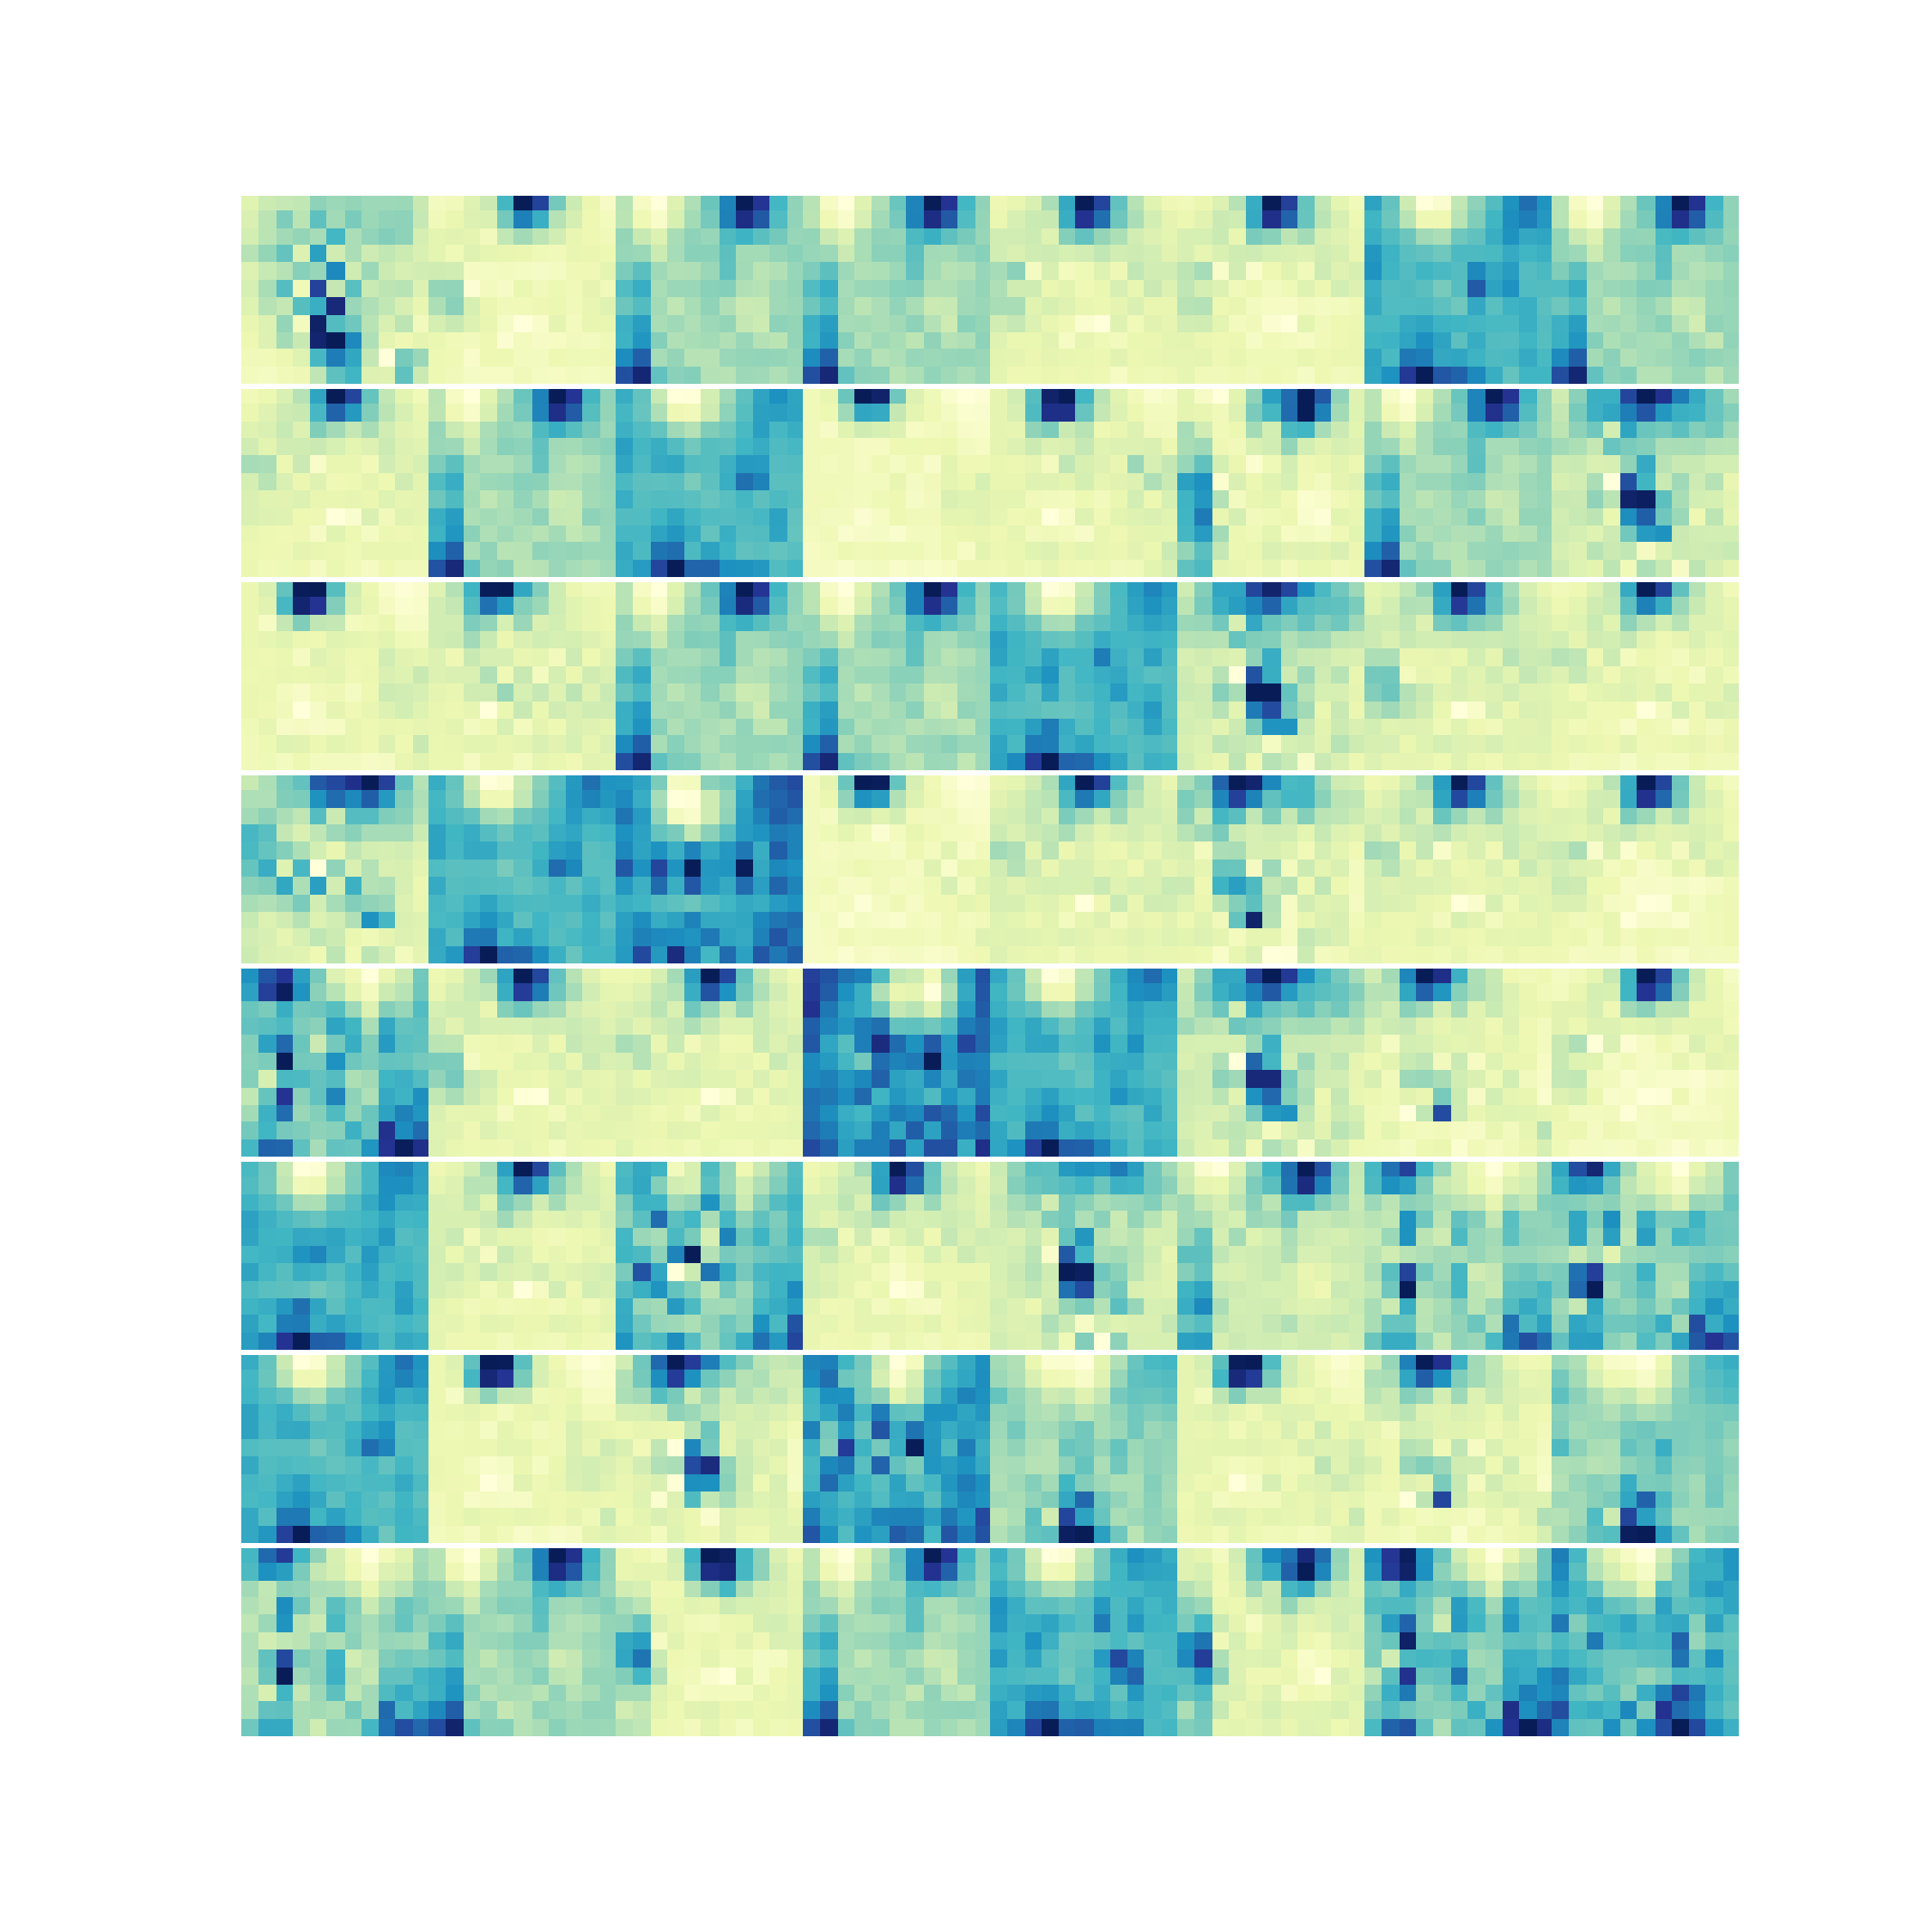
\includegraphics[width=0.45\textwidth]{figures/conv-filts.pdf}
      }
      \subfloat[Convolved Jet Image differences\label{subfig:convolvedfilters}]{
        \includegraphics[width=0.45\textwidth]{figures/newconvos.pdf}
      }
      \caption{Convolutional Kernels (left), and convolved feature differences in jet images (right)}
      \label{fig:convkernels}

    \end{center}
\end{figure}

A related way to visualize the information learned by various nodes in the network is to consider the jet images which most activate a given node.  Fig.~\ref{fig:mostactiviate} shows the average of the 500 jet images with the highest node activation  for the last hidden layer of the MaxOut network (the layer before the classification layer).  The first row of images in Fig.~\ref{fig:mostactiviate} show clear two-prong signal-like structure whereas the second and third rows show one-prong diffuse radiation patterns that are more background-like.  The remaining rows have a variety of $\Delta R$ distances between subjets and have a mix of background and signal-like features.

%For every node in the last hidden layer in the maxout network (i.e., the layer before the classification layer) we examine the node activations, and take the weighted (by pT flat  weights) average of the top 501 jet images that activate that node. Then, we order the nodes from top left to bottom right by increasing sparsity -- that is, we go from least sparse (most commonly activated and > 0) to most sparse (least commonly activated and frequently equal to zero). Fig.~\ref{fig:mostactiviate}.

\begin{figure}[!htbp]
  \centering
  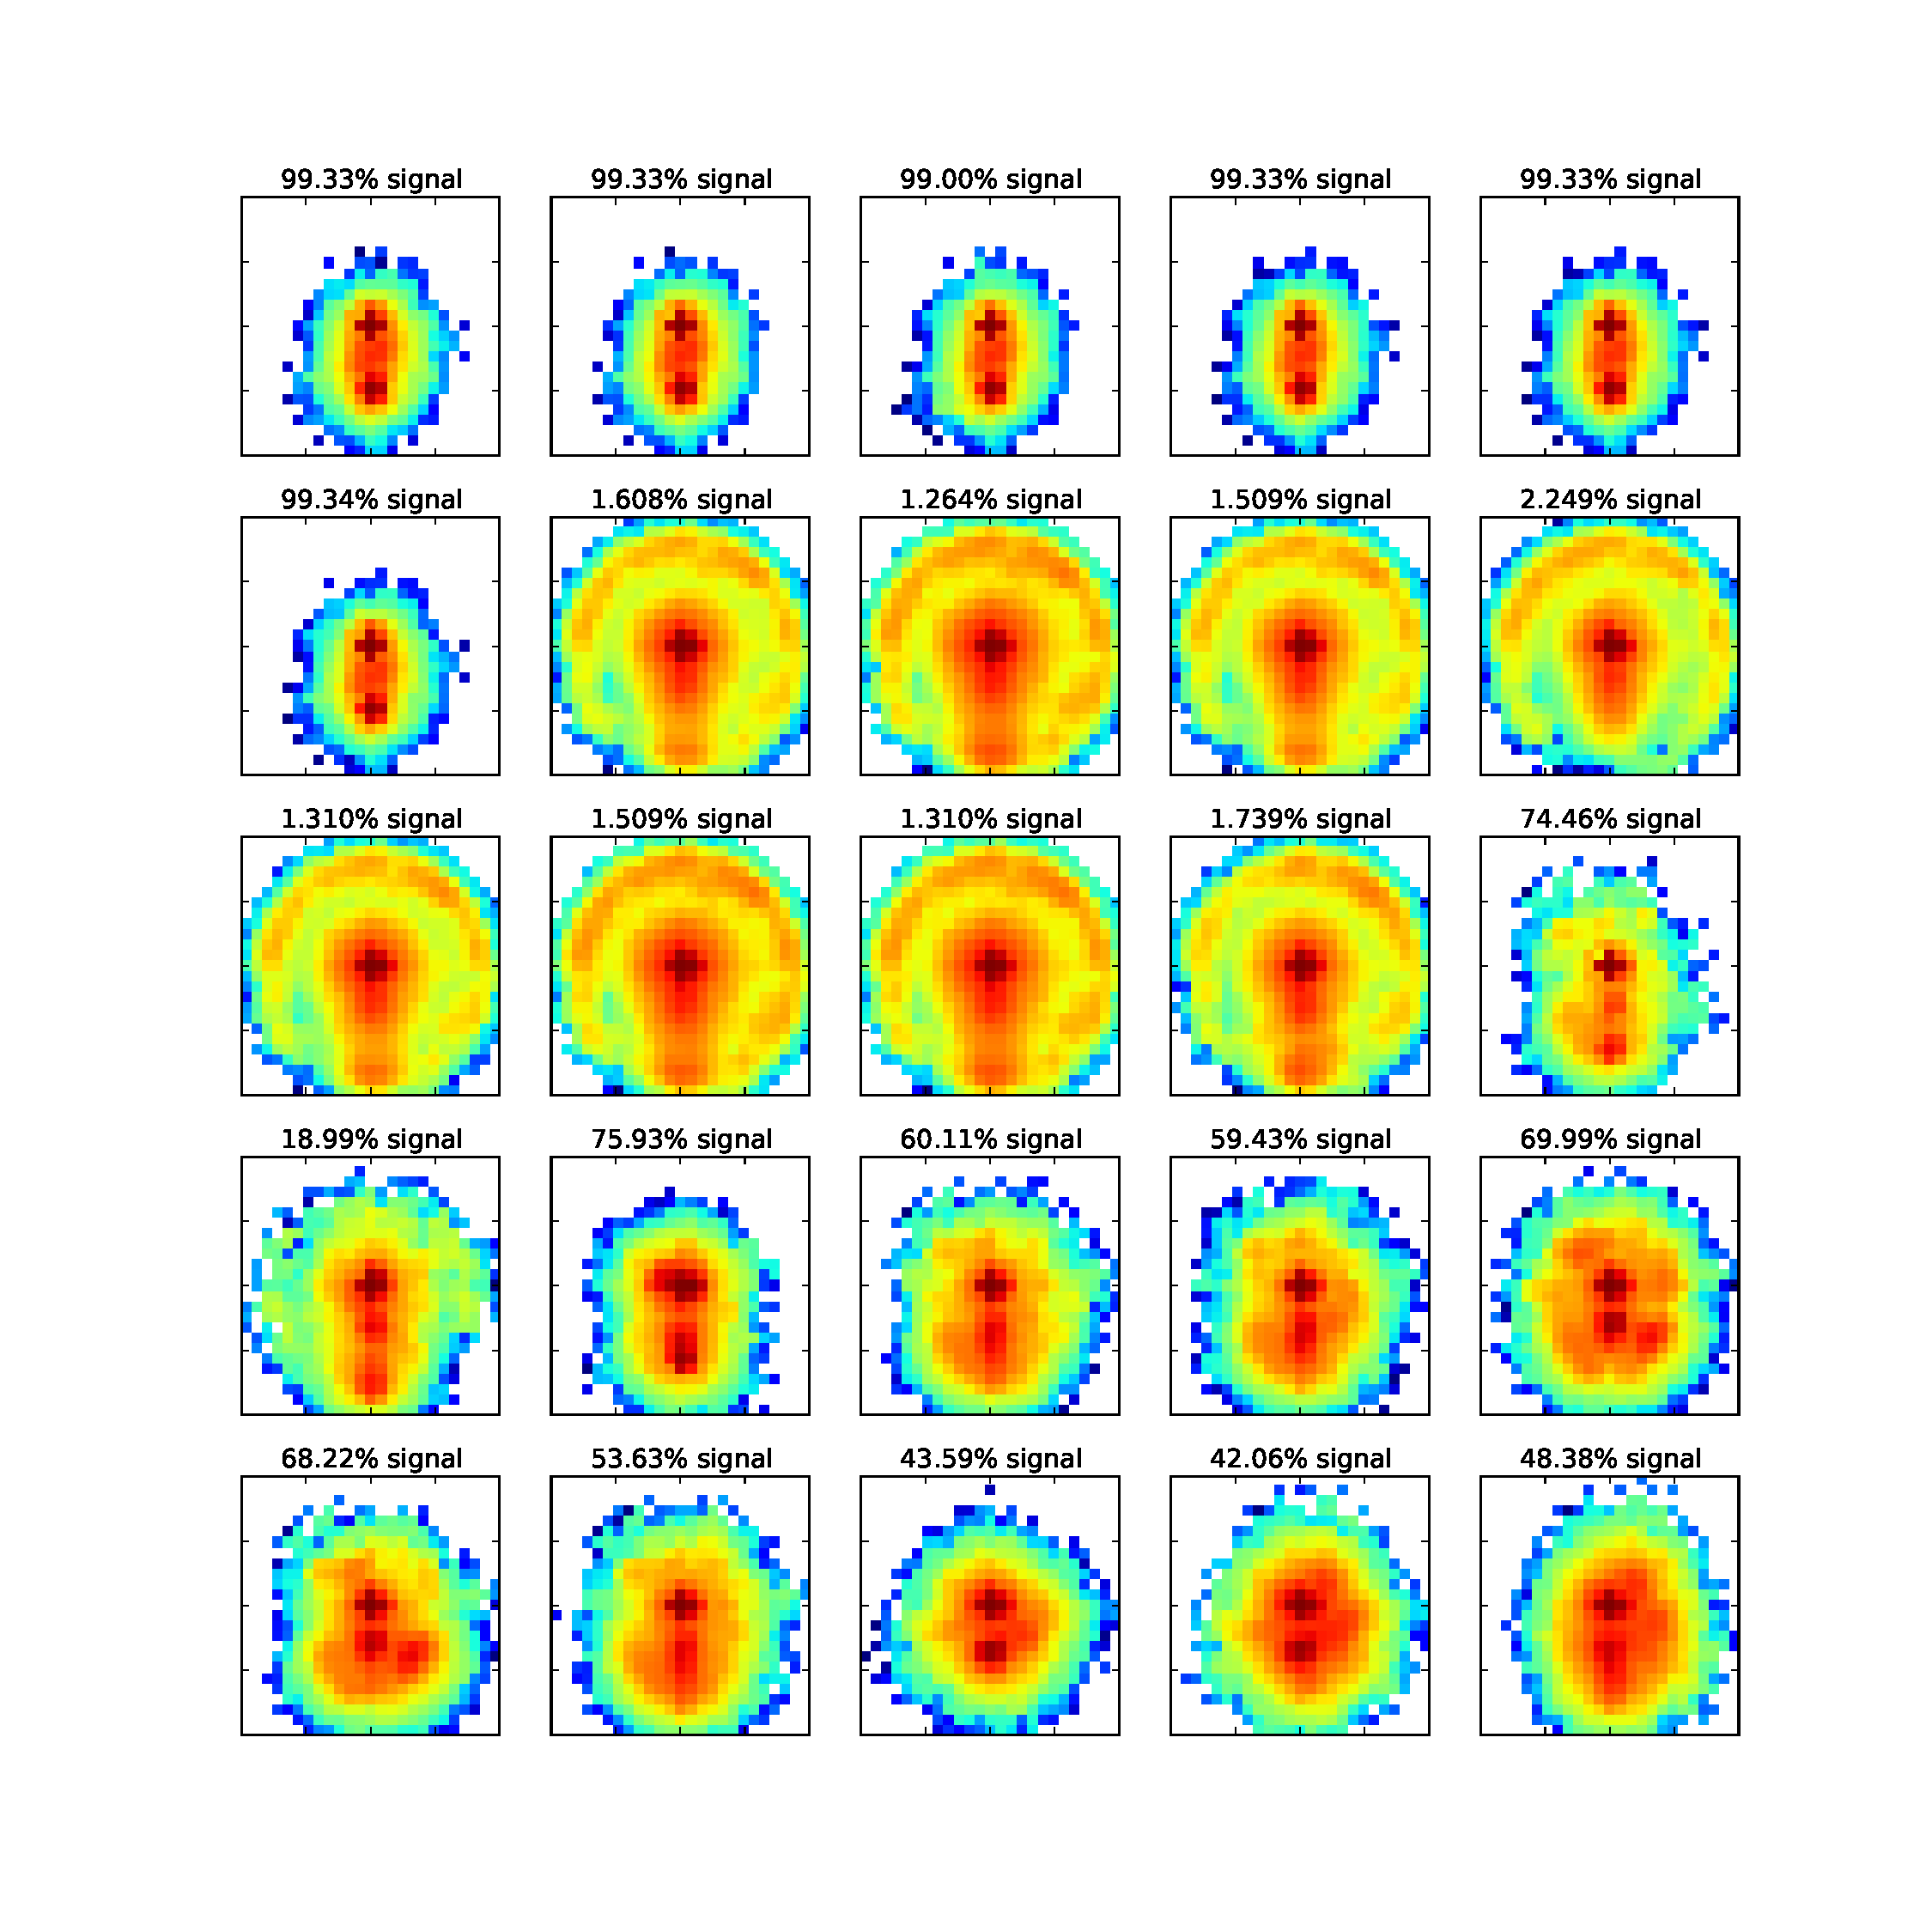
\includegraphics[width=0.8\textwidth]{figures/maxnodes.pdf}
  \caption{The average of the 500 jet images with the highest node activation  for the last hidden layer of the MaxOut network.  The nodes are ordered from top left to bottom right by increasing sparsity.  The top left is the most commonly activated node whereas the bottom right node is least activated and frequently zero. }
  \label{fig:mostactiviate}
\end{figure}


\clearpage
\newpage

\subsection{Physics in Deep Representations} % (fold)
\label{ssub:physics_in_deep_representations}
To get a tangible and more intuitive understanding of what jet structures a DNN learns, we compute the correlation of the Conv-Norm network output with each pixel of the jet-images. Specifically, let $y$ be the DNN output, and consider the intensity of each pixel $I_{ij}$ in transformed $(\eta, \phi)$ space. We the construct an image, which we denote the \emph{deep correlation jet-image}, where each pixel $(i, j)$ is $\rho_{I_{ij}, y}$, the Pearson Correlation Coefficient of the pixels intensity with the final DNN output, across images. While this this image does not give a direct view of the discriminating information learned within the network, it does provide a guide to how such information may be contained within the network.  In Figure~\ref{fig:corr}, we construct this deep correlation jet-image for both the Convnet and the Maxout networks.  We can see that the location and energy of the subleading subjet, found at the bottom of the image, is highly correlated with the DNN output and important for identifying signal jet-images.  In contrast, the information contained in the leading subjet, seen at $(x,y)\sim (0,0)$ in the image, is not particularly correlated with the network owing to the fact that both signal and background jets have high energy leading subjets.  We also see asymmetric regions around both subjets that are correlated with the DNN output and is indicating the presence of additional radiation expected in the QCD background jets.  Finally, a small negative correlation with the rest of the jet area is seen, indicating that radiation from the background jets is more likely to be observed in these regions.   The exact function form of this distribution is not known, nor does it seem to describe exactly any known physics inspired variable.
\begin{figure}[!htbp]
  \centering
%  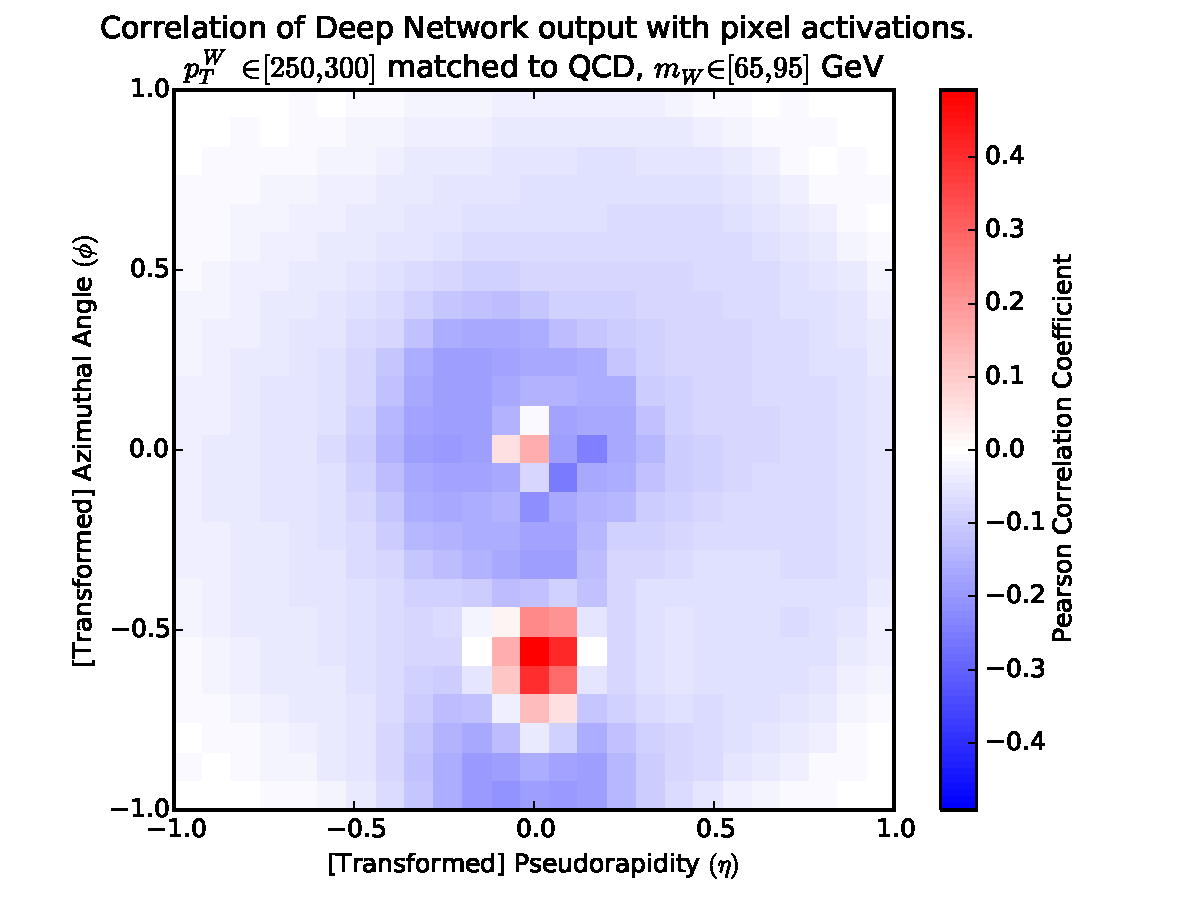
\includegraphics[width=0.5\textwidth]{figures/pixel-activations-corr.pdf}
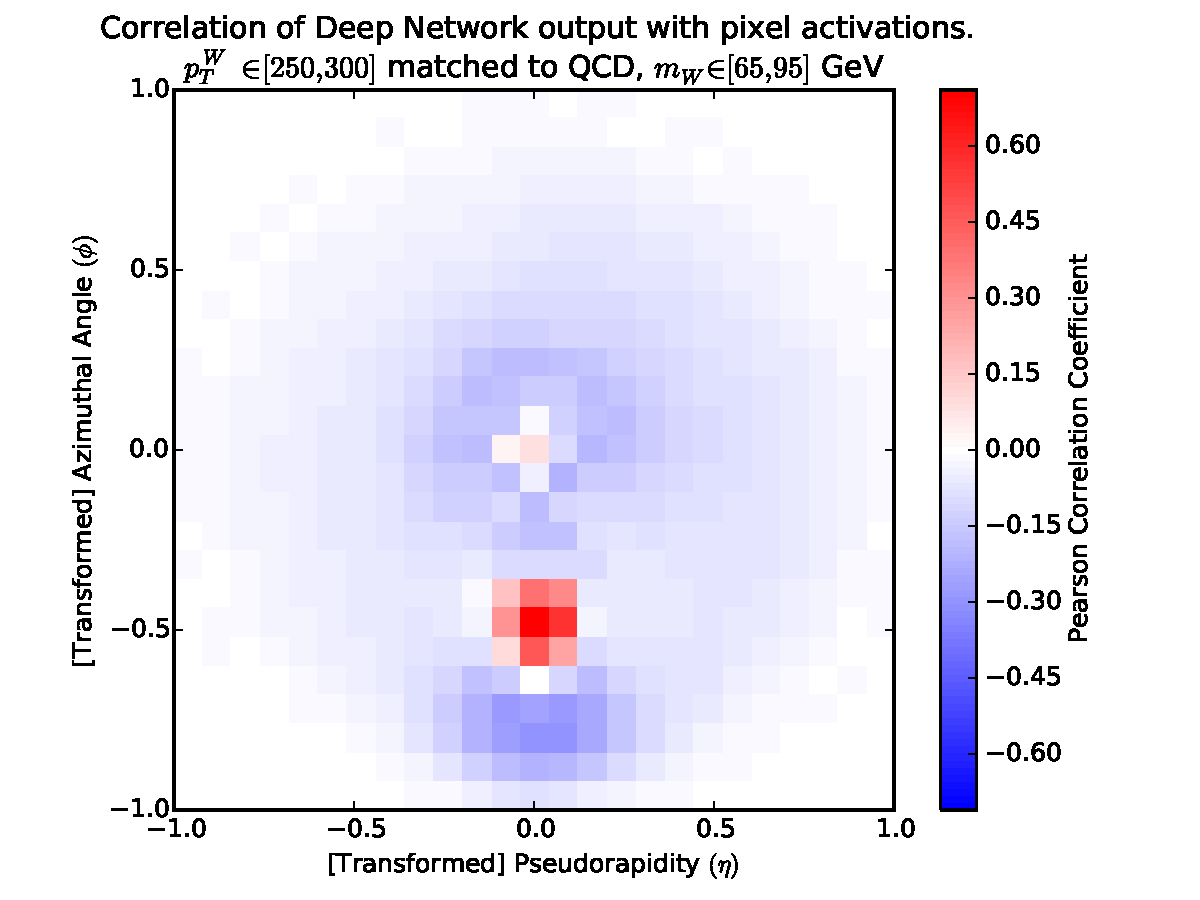
\includegraphics[width=0.5\textwidth]{figures/pixel-activations-corr-cnn.pdf}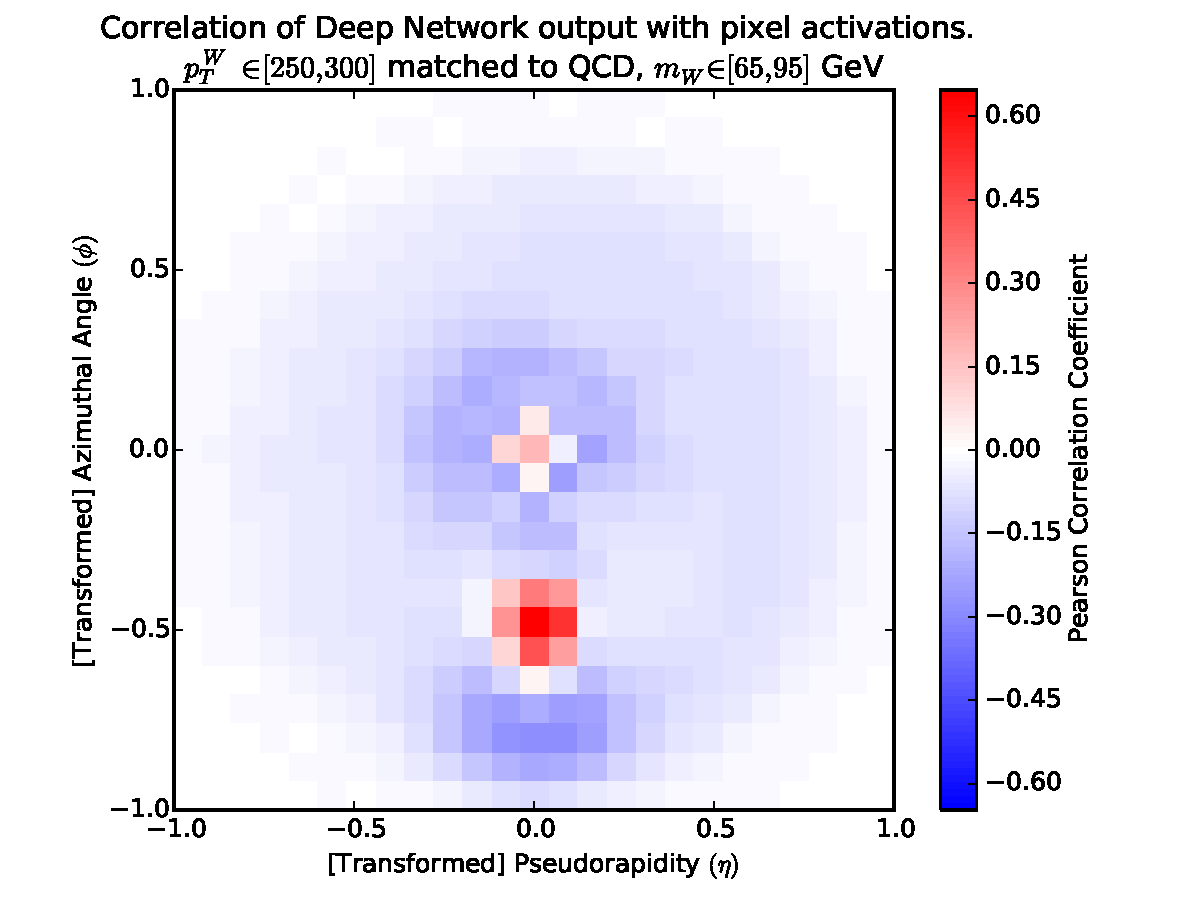
\includegraphics[width=0.5\textwidth]{figures/pixel-activations-corr-maxout.pdf}
  \caption{Per-pixel linear correlation with DNN output for the Convnet (left) and the MaxOut network (right).  Signal and background jets are combined.}
  \label{fig:corr}
\end{figure}

